%%%%%%%%%%%%%%%%%%%%%%%%%%%%%%%%%%%%%%%%%%%%%%%%
%%%%%%%%%%%%%Przykładowy dokument%%%%%%%%%%%%%%%
%%%%%%%%%%wraz z klasą pracadyp.cls%%%%%%%%%%%%%
%%%%%%%%%%%%%%%%%%%%%%%%%%%%%%%%%%%%%%%%%%%%%%%%

% w nawiasie kwadratowym wpisujemy rodzaj pracy: 
% magisterska, licencjacka, inzynierska
\documentclass[licencjacka]{pracadypl}


%% ważne definicje %%
\usepackage{tgtermes}
\usepackage[T1]{fontenc}
\usepackage{polski}
\usepackage[utf8]{inputenc}
\input glyphtounicode
\pdfgentounicode=1
\usepackage{amssymb}
\usepackage{amsmath}
\usepackage{graphicx}
\usepackage{titlesec}
\usepackage{color}
\usepackage{xcolor}
\usepackage{float}
\usepackage{tablefootnote}
\usepackage{hyperref}
\usepackage{titling}
\usepackage{interval}
\bibliographystyle{plain}

\def\mgr{magisterska}
\def\lic{licencjacka}
\def\inz{inżynierska}

\def\sk{Słowa kluczowe}
\def\kw{Keywords}
\def\et{Title in English}
%% koniec ważnych definicji %%



%% wypełnia Autor pracy %%

%autor pracy
\author{Kajetan Owczarek}
%numer albumu
\nralbumu{396396}
%tytuł pracy
\title{Przykłady zastosowania technik optymalizacji czasu wczytywania witryny internetowej}
%kierunek studiów
\kierunek{Informatyka}
%promotor w dopełniaczu
\opiekun{prof. dr Wojciecha Horzelskiego}
\katedra{Katedra Informatyki Stosowanej}
%rok
\date{2023}
%Słowa kluczowe:
\slkluczowe{pierwsze, drugie, trzecie, czwarte}
%tytuł po angielsku
\tytulang{Title in English}
%słowa kluczowe po angielsku
\keywords{first, second, third, fourth}
%% koniec ważnych definicji %%

%% APD %%
%% w systemie APD należy jeszcze wpisać, poza powyższymi informacjami, streszczenie oraz streszczenie w języku angielskim  %%


%%% definicje %%%
\def\pd{\noindent \textbf{Dowód.~}} %%początek dowodu
\def\kd{\hfill\mbox{$\rule{2mm}{2mm}$}} %%koniec dowodu
\newtheorem{defi}{Definicja}[section]
\newtheorem{uwaga}{Uwaga}[section]
\newtheorem{tw}{Twierdzenie}[section]
\newtheorem{lem}{Lemat}[section]
\newtheorem{wn}{Wniosek}[section]
\renewcommand\thetw{\thesection.\arabic{tw}.}
\renewcommand\thedefi{\thesection.\arabic{defi}.}
\renewcommand\theuwaga{\thesection.\arabic{uwaga}.}
\renewcommand\thetw{\thesection.\arabic{tw}.}
\renewcommand\thelem{\thesection.\arabic{lem}.}
\renewcommand\thewn{\thesection.\arabic{wn}.}
%
\definecolor{wmiigreen}{rgb}{0.0, 0.5, 0.0}
\titleformat{\chapter}[display]
  {\normalfont\huge\bfseries\color{wmiigreen}}{\chaptertitlename\ \thechapter}{10pt}{\Huge}
 %
\linespread{1.3}
%%% koniec definicji ze wzorca %%%


%%% osobiste definicje

\newcommand{\selfnote}[1]{\colorbox{pink}{#1}}
\hypersetup{
  colorlinks=false,
  linkcolor=red,
  pdftitle={\thetitle},
  pdfborder={0 0 0}
}
\intervalconfig{
  soft open fences
}

%%% koniec definicji

\begin{document}

\maketitle
\tableofcontents
\newpage



\chapter{Wstęp}

Pomimo nieustającego rozwoju technologii telekomunikacji oraz zwiększania prędkości łączy internetowych, problem wydajności usług internetowych nie zniknął, ani nie zapowiada się, aby tak się zadziało. Od potrzeb łączności poza terenami zabudowanymi, przez starzejący lub ograniczony sprzęt, po malejącą cierpliwość użytkowników, rozważanie, jak najszybciej dostarczyć treści z serwera do urządzenia użytkownika jest powszechne w pracy ze stronami internetowymi.

Celem tej pracy jest zaprezentowanie serii technik i optymalizacji, pozwalających na poprawienie czasów wczytywania witryn internetowych na urządzeniach użytkownika, oraz porównanie ich przy pomocy obiektywnych i powszechnie stosowanych narzędzi i metryk.

Celem zilustrowania efektów takich optymalizacji, a w szczególności wpływ ich braku na używalność strony, zaprezentuję przykładową stronę zrobioną przy użyciu najprostszych, najpopularniejszych technik. Celem moim jest stworzenie strony, która zrobiona jest kompetentnie, acz z zerową uwagą przyłożoną do wydajności strony pod względem wczytywania i procesu uruchamiania strony. Następnie, poprzez stosowanie technik wpływających minimalnie na funkcjonalność strony, poprawiać wyniki pomiarów obiektywnych.

\chapter{Sposób pomiarów}
Celem usunięcia jak najwięcej zewnętrznych zmiennych w danych pomiarowych,
% \footnote{Choć dla porównania wydajności wyniki z jednej maszyny powinny wystarczyć, niestety zaobserwowałem znaczne, trudne do zrozumienia fluktuacje wydajności mojego komputera. Wyniki na nim były by więc wewnętrznie niespójne.}
skorzystam z narzędzia używanego powszechnie w branży, którym jest WebPageTest.

WebPageTest to operowana przez firmę Catchpoint usługa, pozwalająca na wykonanie dokładnego pomiaru wczytywania strony w wybranym regionie, na emulowanym urządzeniu, w określonych warunkach sieciowych. Używając standaryzowanego środowiska, możemy usunąć wiele zmiennych wynikających z aktywności innych aplikacji na testującej maszynie oraz innych urządzeń w sieci. Sprawia to też, że wyniki są o wiele bardziej uniwersalne - mogąc odnieść się do środowiska ze znanymi charakterystykami wydajności, można usunąć element niepewności i zgadywania, na ile aplikowalne są dla naszych rozważań czyjeś wyniki. 

WebPageTest dostarcza dokładny zapis procesu wczytywanie naszej witryny. Dane te są prezentowane w formie złożonego wykresu, o którym opowiem więcej w późniejszym rozdziale, kiedy zajmiemy się porównywaniem wydajności przed i po zastosowaniu technik.

Rozważałem wcześniej użycie do pomiarów stworzonego przez Google narzędzia o nazwie Lighthouse, które stara się spełnić podobną funkcję oceny wydajności, acz analizuje też wiele innych metryk dotyczączych rzeczy jak używanie technologii pomagających osobą używającym czytników ekranu, optymalizacji pod kątem wyszukiwarek internetowych, czy współczesności strony. Niestety, sposób działania Lighthouse'a jest ograniczony w swojej dokładności. Zamiast dokonywać pełnej symulacji wydajności standardowego urządzenia, dokonuje on testy w pełnej prędkości, a następnie przeskalowując je. Tak jak nie jest to zła metoda żeby optymalizować lokalnie, gdyż Lighthouse sugeruje też sposoby poprawy, tak użycie go nie eliminuje częściowej zmienności wynikających z natury maszyny, na którym są dokonywane pomiary.

\chapter{Startowy projekt}
Żeby zilustrować techniki, które zostaną omówione później, oraz ich wpływ na wydajność wczytywania strony, potrzebna jest na to przestrzeń w formie przykładowej witryny. Tworząc ją, celowałem w popełnienie prostych do popełnienia błędów, oraz decyzje niesprzyjające czasowi wczytywania. Stworzyłem więc udawaną stronę z wiadomościami. Zawiera ona niemałą ilość zdjęć, dużo tekstu, oraz parę elementów interaktywnych. 

\begin{figure}[H]
  
\includegraphics[width=\linewidth]{images/frontpage.png}
  \caption{Nagłówek strony, karuzela z wiadomościami}
  \label{fig:frontpage}
\end{figure}

\begin{figure}[H]
  
\includegraphics[width=\linewidth]{images/frontpage-articles.png}
  \caption{Fragment listy artykułów}
  \label{fig:frontpage-articles}
\end{figure}

\begin{figure}[H]
  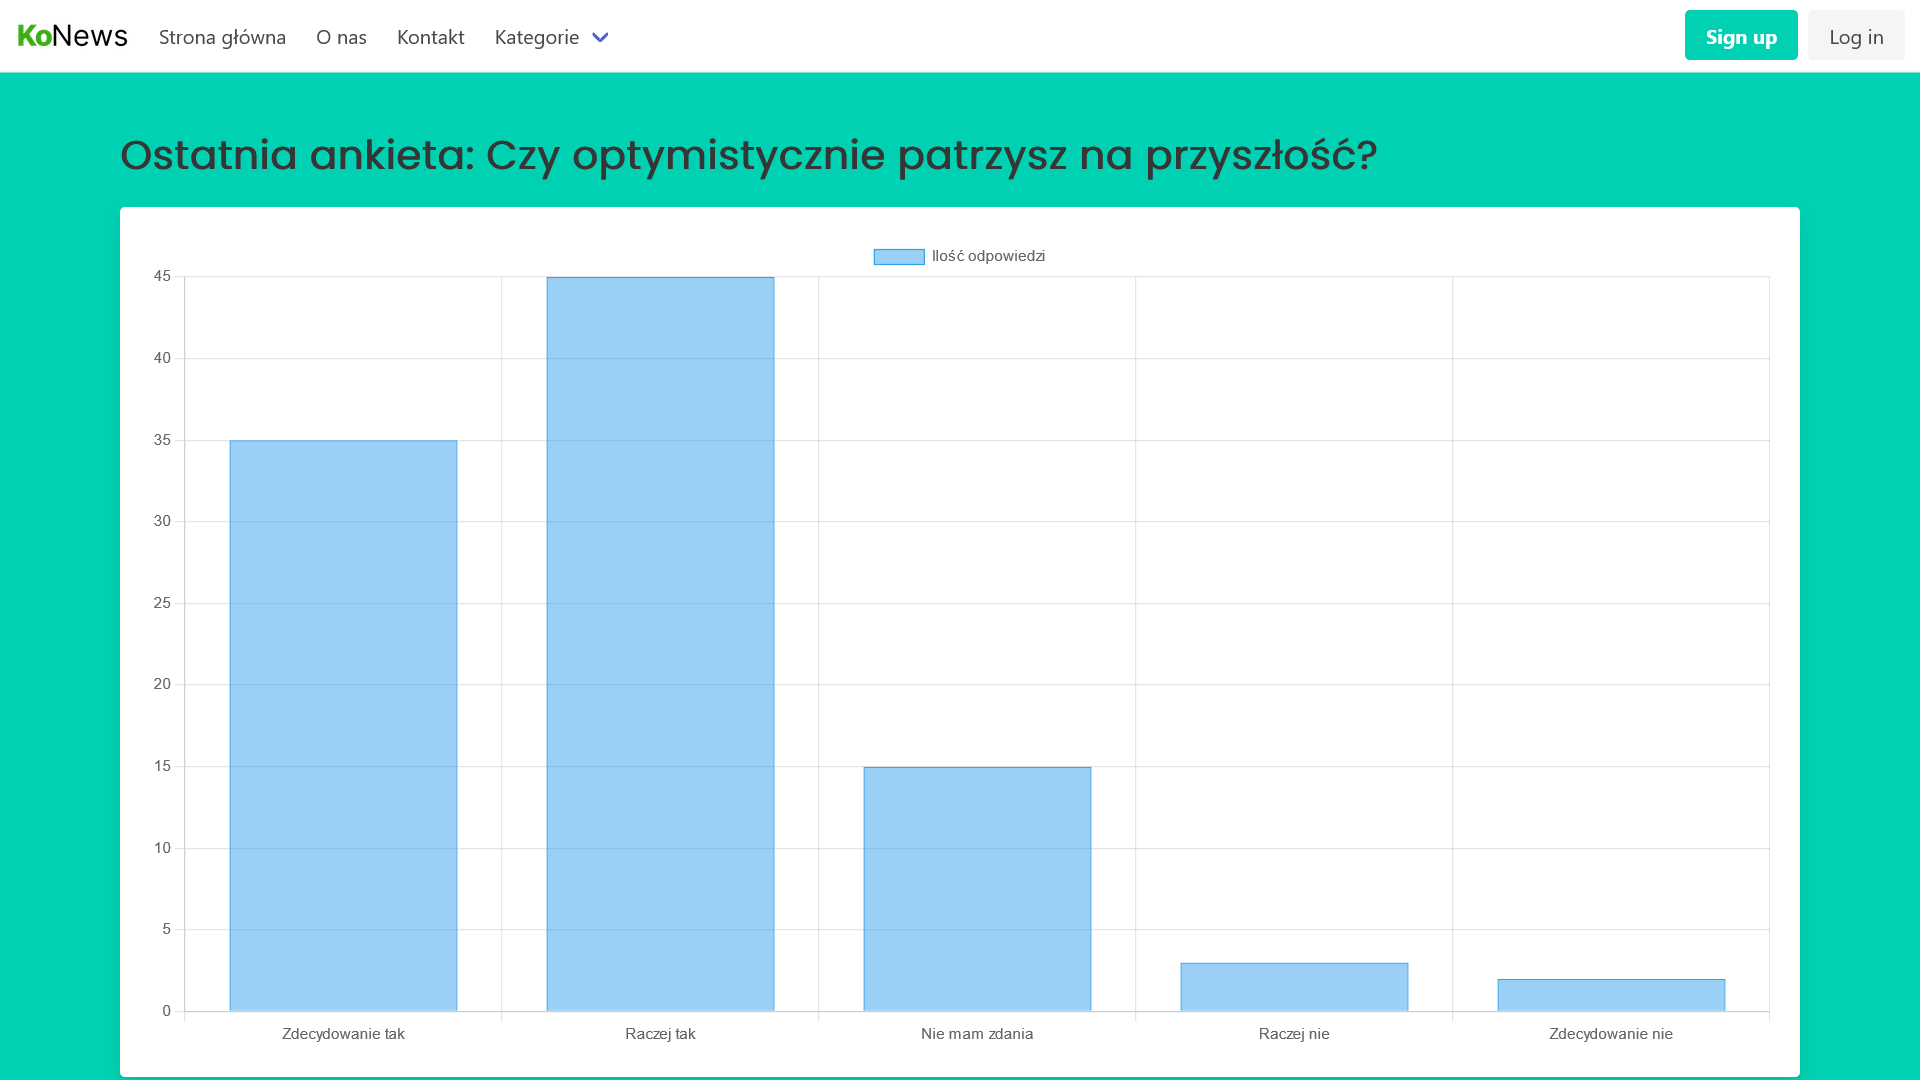
\includegraphics[width=\linewidth]{images/frontpage-dynamic-article.png}
  \caption{Dynamiczne treści - wyniki ankiety w wykresie}
  \label{fig:frontpage-dynamic}
\end{figure}

Żeby zaprezentować efekty dużej ilości treści w dokumencie HTML, dodałem do niej jedno ze źródeł do treści tu zawartej, czyli specyfikację parsowania dokumentów HTML.

\begin{figure}[H]
  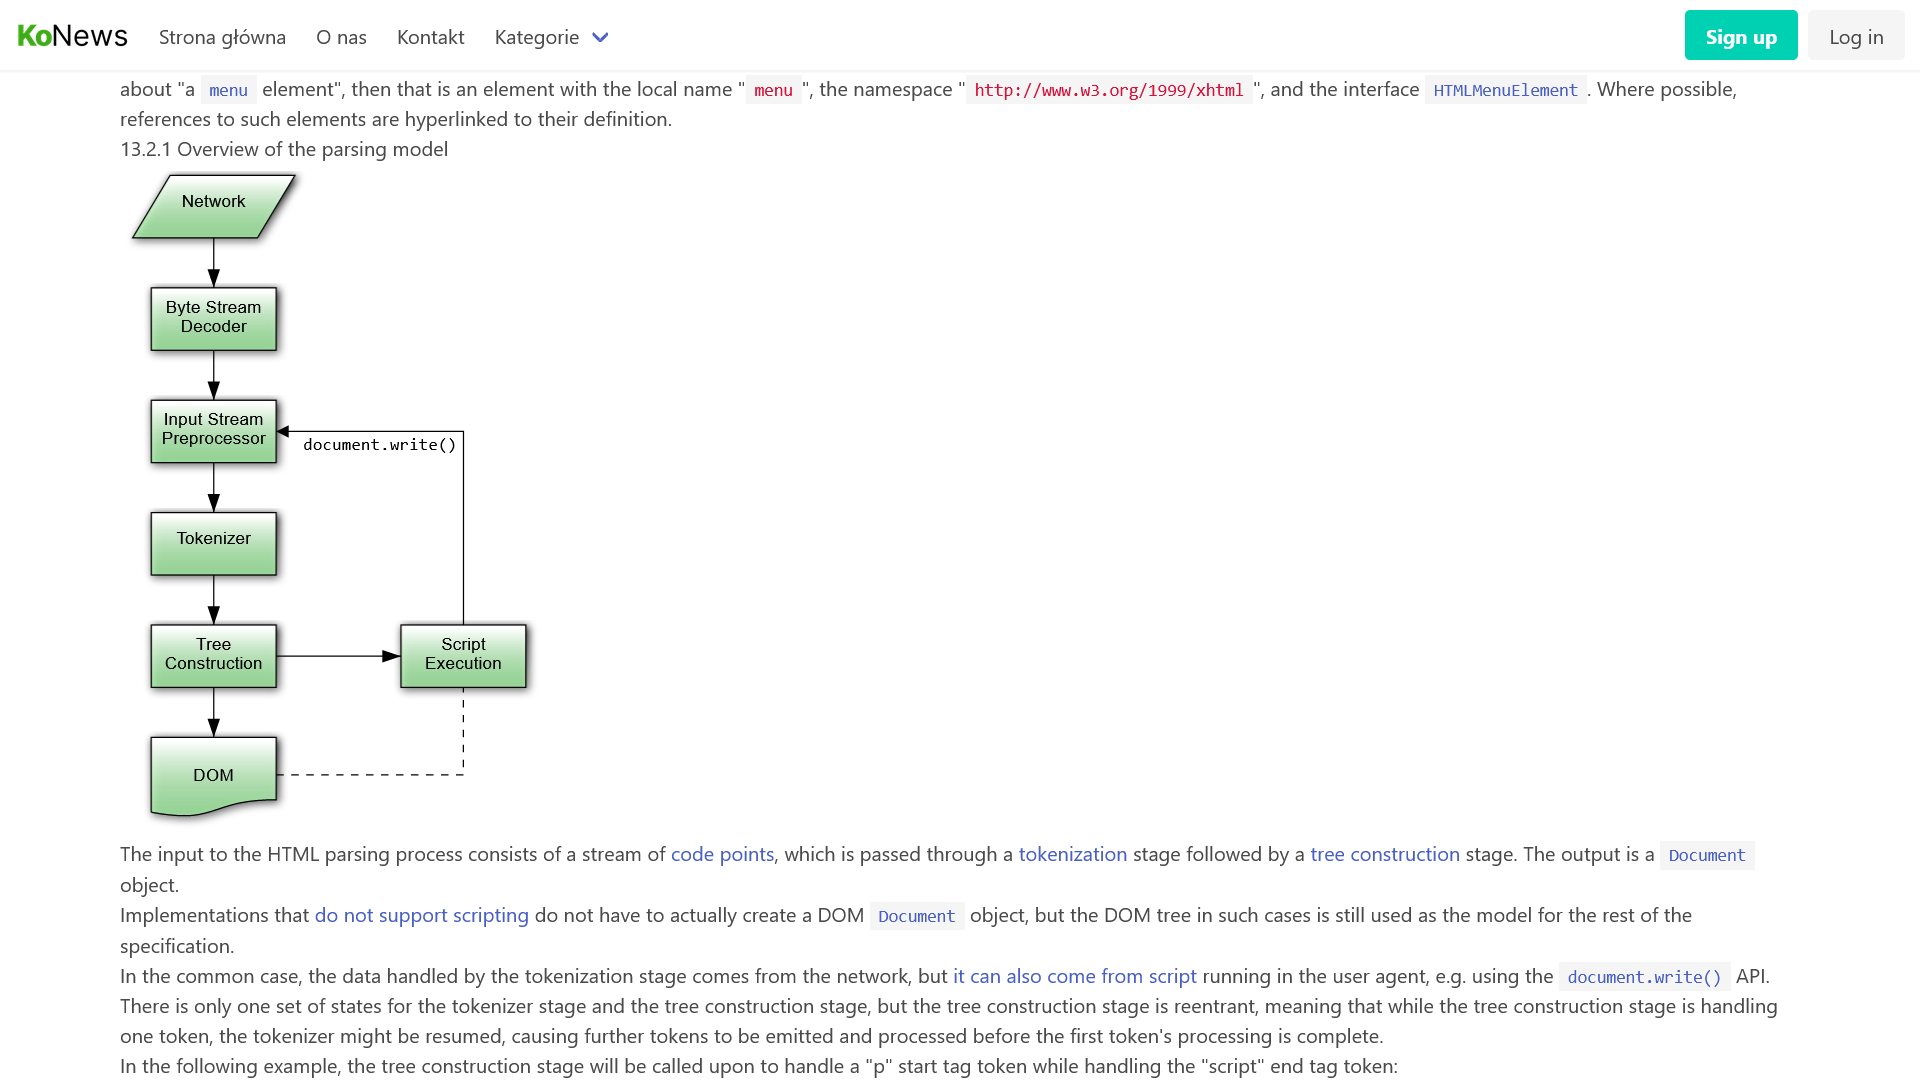
\includegraphics[width=\linewidth]{images/frontpage-spec.png}
  \caption{Duże treści - specyfikacja parsowania HTML}
  \label{fig:frontpage-spec}
\end{figure}




\chapter{Wstępna analiza wydajności}
Zanim zaczniemy poprawianie naszej witryny, powinniśmy zbadać, jak zachowuje się nasz projekt startowy. Optymalizując na ślepo, jest prosto zmarnować czas przyśpieszając elementy, nie zmieniając finalnej wydajności\footnote{W przypadku tworzenia witryn internetowych jest to szczególnie prosty do popełnienia błąd. Interakcja równoległego wczytywania zasobów, oraz mechanizm zasobów blokujących może sprawić, że dowolne przyśpieszenie jednej cześci nie wpłynie zupełnie na finalną szybkość wczytania, gdyż całość przeglądarki będzie czekało na inny element.}. Głownym wynikiem wykonywania analiz przy pomocy WebPageTest'u jest wykres zwany waterfall'em, czyli wodospadem. Jest on bardzo gęsty w dane i zawiera przede wszystkim dane o połączeniach sieciowych oraz stanie przeglądarki. Omówię po krótce jak go odczytywać\footnote{Dostepna na stronie WebPageTest'u lekko interkatywna wersja tego wykresu pozwala odczytać te dane nieco prościej, oraz daje dostęp do dodatkowych informacji, których nie ma na obrazkowym waterfall'u.}, równocześnie zwracając uwagę na problemy, które można zobaczyć ze wstępnych testów;
\begin{figure}[h!]
  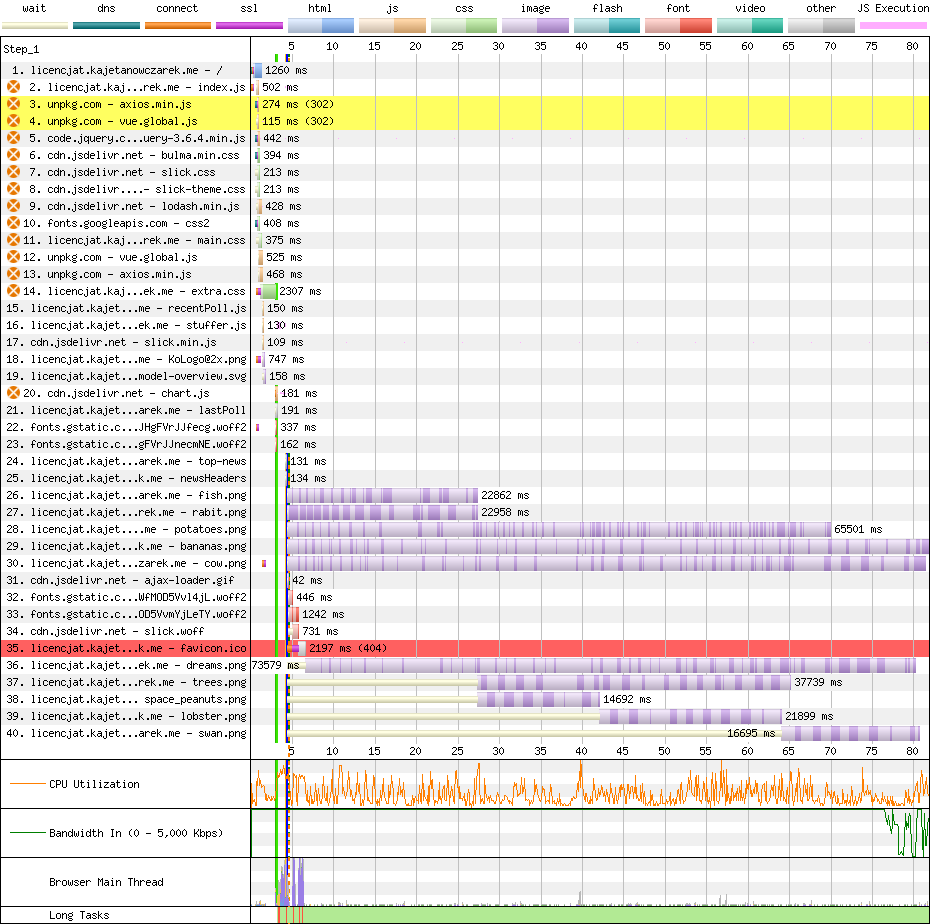
\includegraphics[width=\linewidth]{images/base-waterfall-all-final.png}
  \caption{Wykres produkowany przez WebPageTest, zwany jako Waterfall}
  \label{fig:waterfall-base}
\end{figure}
Na górze wykresu znajduje się legenda, informująca nas, które kolory na wykresie oznaczają jaką fazę rozpoczynania połączeń, oraz rodzaje treści przez te połączenia przesyłane. 

Tuż pod nią, znajduje się głowna część, która zawiera najważniejsze dane, czyli wykres rozkładu czasowego realizacji kolejnych zapytań wykonywanych przez naszą przeglądarkę. Od góry do dołu mamy zapytania HTTP, od rozpoczętego najwcześniej do najpóźniej, natomiast od lewej do prawej mamy upływ czasu. Same okresy, kiedy zapytania naszej witryny były realizowane, są zaznaczone jako prostokąty na wykresie. Poprzez cienkie prostokąty są zaznaczane obszary czasu, kiedy połączenia nie postępowały stan wczytania naszej strony, specyficznie otwieranie połączeń i wykonywanie kodu JavaScript. Grubymi prostokątami jest za to zaznaczone, kiedy treści rzeczywiście były pobierane, na blado kiedy połączenie jest otwarte, ale nie są przesyłane dane, oraz na mocniejszy kolor, kiedy miało miejsce przesyłanie na łączu danych.

Poniżej głownego wykresu, mamy informacje o zużyciu mocy procesora. W naszym przypadku nie będziemy mieli wiele okazji żeby skorzystać z tych danych, ale jest to możliwe, że dokonywanie dużej ilości obliczeń będzie opóźniać naszą witrynę, i wtedy to na tym wykresie to zobaczymy.

Jeszcze niżej, znajduje się wykres zużycia łącza. Im linia na nim jest wyżej, tym więcej dostępnego naszemu testowem urządzeniowi łącza wykorzystujemy. W większości sytuacji chcemy, żeby nasza linia była jak najwyżej, gdyż to oznacza, że ograniczają nas zewnętrzne warunki sieciowe, a nie nasze własne urządzenie.

Przedostatni wiersz jest zajęty przez wykres przetwarzania wykonywanego przez przeglądarkę. Wysokością przedstawia on, jak bardzo zajęty jest główny wątek przeglądarki (pełny na wysokość znaczy, że pętla wydarzeń przeglądarki była w pełni zajęta), natomiast kolor sygnalizuje, jakie działania dominowały w danym momencie.

Ostatnim, zarazem najważniejszym i najmniej ważnym, jest wykres interaktywności. Na biało oznaczony jest czas, zanim strona była użytkownikowi wyświetlona, na czerwono kiedy przeglądarka była zbyt zajęta, by reagować na wejścia, a na zielono, kiedy wszystko działało. Tak jak wykres ten ilustruje bardzo ważny aspekt działania strony - dominacja czerwieni oznacza, że dla użytkownika wszystko wydaje się zacięte - tak nie daje on informacji, czemu tak się dzieje, oraz sugestii co można zmienić. Na szczęście wykres tuż nad nim bardzo silnie przekłada się na interaktywność, więc można traktować je jako wspólną część, górny jako dokładną wartość, dolny jako miarkę, czy przekroczyliśmy punkt upadku używalności. 

Prócz tego, przez cały wykres przebiega kilka pionowych linii, które oznaczają kluczowe momenty we wczytywaniu strony, jak kiedy użytkownikowi wyświetliło się na ekranie cokolwiek, kiedy strona mogła po raz pierwszy reagować na wejścia użytkownika, czy kiedy nastąpiła największa zmiana wyglądu. Na tej wersji wykresu nie widać ich zbyt dobrze, gdyż wszystkie oznaczane tak wydarzenia zdarzyły się względnie wcześnie. Jednakże, na późniejszych wersjach wykresów, będziemy mogli używać ich, żeby znajdywać najważniejsze punkty, które chcemy, aby wydażały się jak najwcześniej.

Wiedząc już, co oznaczają części naszego waterfall'a, możemy zauważyć, że wczytywanie naszej strony dominuje parę jasnofioletowych fioletowych zapytań. Korzystając z legendy i zrozumienia, jak wykres ten czytać, wiemy, że są to zdjęcia, które wczytują się długo, i intensywnie walczą o użycie łącza. Tak samo patrząc na zieloną kreskę wykresu przepustowości łącza widzimy, że używamy całość przydzielonego nam łącza przez większość czasu wczytywania strony. Nie jest to zła rzecz, bo to znaczy, że nasza strona może wczytywać się szybciej, o ile tylko dostanie szybsze połączenie.

Zacznijmy więc optymalizować nasz projekt.

\chapter{Optymalizacja witryny}
\section{Kompresja}
Najprostrzmy sposobem, aby dodać niesłychaną ilość rozmiaru dowolnemu projektowi komputerowemu, to użycie nieskompresowanych zasobów w dużej rozdzielczości. Dla przykładu, rozdzielczość FullHD, czyli $1920\times1080\left(=2073600\right)$ pikseli, współcześnie bardzo powszechną w każdej klasie jakościowo-cenowej\footnote{Wg Steam Hardware Survey, ponad 66\% użytkowników platformy Steam posiada właśnie taką rozdzielczość na swoim głównym monitorze. Choć dane tej platformy }, o standardowej formie zapisu koloru pikseli, czyli 3 kanały, po 8 bitów na kanał, daje $2073600\times3\times8 = 49766400$ bitów, czyli $49.77$ megabitów. Mając dostępny przeciętny polski internet, który według statystyk firmy Ookla\footnote{Dane wzięte z \url{https://www.speedtest.net/global-index/poland}} jest w stanie pobrać $107.85$ megabitów na sekundę, pobranie jednego, nieskompresowanego zrzutu ekranu zajęłoby $461$ milisekund. Gdybyśmy więc chcieli po prostu przesłać użytkownikom naszej strony całoś ekranu, który mają widzieć, to bez użycia żadnych optymalizacji przeciętne doświadczenie użytkownika to nieco ponad dwie klatki na sekundę płynności.

Niezmiennie, usługi jak filmy czy seriale online, udostępnianie ekranu na komunikatorach jak Teams czy Discord, lub telekonferecjowanie w dużych grupach z wysokiej jakościami kamerkami jakoś obchodzą ograniczenia prędkości przesyłów i rozmiaru zdjęć i wideo. 
Kluczem do osiągnięcia tej niemożliwości jest kompresowanie przesyłanych danych. Technik na takowe jest wiele, i zależne od zawartości transmitowanych informacji. Uniwersalnie, możemy użyć algorytmów bezstratnej kompresji danych, jak LZ77 czy kodowanie Huffmana, aby wykorzystać statystyczne właściwości naszych danych, by usunąć niewydajności w naszym zapisie surowych bajtów naszej treści. Dla specyficznych treści, jak te, które na końcu są odbierane przez ludzką percepcję, możemy często usunąć wiele nieważnych detali, jak dokładne wartości każdego z pikseli czy każdą częstotliwość dźwięku, aby stworzyć o wiele mniejszy plik, który jest tylko delikatnie innym doświadczeniem dla odbiorcy. Pewnego rodzaju kompresją może też być samo tworzenie programów - tak jak opisany wcześniej przykład przesyłania każdej klatki na urządzenie użytkownika jest niemożliwe, tak wysłanie programu, który będzie generował nowe klatki z wielkim tempem, korzystając z ogromnych możliwości przetwarzania i przemieszczania danych wewnątrz współczesnych komputerów, jest współcześnie niemalże trywialnie proste.

Skorzystajmy więc z technik kompresji, żeby poprawić znacznie czas wczytywania naszej witryny.

\section{Kompersja zdjęć}

\selfnote{Czasem fancier formty z większym przetwarzniem tworrzą większe zdjęcia.}

Dzięki użyciu poprawnie kompesji możemy znacznie zmniejszyć rozmiar plików ze zdjęciami. Nasz projekt w podstawowej wersji przesyłał $46.6$MB zdjęć, co przy prędkości łącza $5000$Kbps oznacza około 1 minutę i 15 sekund pobierania, co zgadza się z naszymi testami - pierwsze zdjęcie zaczyna pobierać się nieco przed piątą sekundą, a wczytywanie kończy się koło 82 sekundy. Zdjęcia te były zapisane w formacie PNG, który wspiera tylko bezstratną kompresję\footnote{PNG: The Definitive Guide - ISBN 1-56592-542-4, 1.2.4}, i choć wiele pracy zostało włożone, żeby wykorzystać ją najlepiej jak się da, od pewnego momentu po prostu nie jesteśmy w stanie nie zapisać jakoś danych zawartych na zdjęciu. Głównym założeniem formatu PNG to kompatybilość i edytowalność w pełnej jakości, więc jeżeli chcemy rozmiaru, musimy poszukać innego formatu.

W momencie pisania tego dokumentu, istnieją trzy formaty zdjęć, które konkurują o rolę preferowanego formatu dla obrazów w internecie. Są nimi AVIF, JPEG XL oraz WebP. 

AVIF to format pliku oparty na kodeku wideo AV1, który jest tworzony przez Alliance for Open Media, czyli konsortium największych korporacji oraz projektów open-source. AVIF pozwala na osiągnięcie bardzo małych plików kosztem wielkiej straty jakości, lub dobrą jakość przy średnim, acz lepszym niż dla innych formatów rozmiarze. Niestety, choć za projektem stoją największe jednostki w świecie multimediów, przez nowość tego formatu wsparcie jest dobre, ale dalej z dużymi dziurami. Dodatkowo, konsekwencją bycia pochodną formatu przeznaczonego dla wideo jest to, że AVIF nie posiada możliwości renderowania progresywnego - zdjęcie jest albo w pełni wyświetlone, albo nie jest wyświetlane wcale, więc na wolnym łączu przez cały proces wczytywania zdjęcia nie wyświetla się użytkownikowi cokolwiek. Tak więc jak jest to definitywnie dobra opcja do rozważenia, tak w ramach tego projektu nie skorzystam z AVIF'a.

JPEG XL jest aktywnie rozwijanym następcą używanego powszechnie formatu JPEG. Oferuje szeroki zakres możliwości, jak HDR, większa głębia bitów obrazu, animacje, warstwy i wiele więcej, jednocześnie oferując niesłychanie wydajną kompresję stratną, która w niewielkiej ilości danych oferuje bardzo dobrze wyglądający obraz. Niestety, przez nowość formatu, obsługa takowego jest niemalże zerowa - jedynie parę nowych albo specjalistycznych aplikacji obsługuje ten format, więc w momencie pisania nie jestem w stanie użyć takowego, lecz kiedy pojawi się lepsze wsparcie, zapewne byłby najpraktyczniejszą opcją do użycia.

WebP to stworzony przez Google format, który powstał poprzez wykorzystanie części formatu wideo WebM, aby zapisywać pojedyńcze klatki, więc zdjęcia. Z tej trójki formatów jest on najstarszym, mając przynajmniej dekadę przewagi nad pozostałymi dwoma konkurentami, więc wsparcie wśród przeglądarek jest o wiele większe. Pomimo bycia byłym elementem systemu kodowania wideo, nie ma tego samego problemu z brakiem progresywnego wczytywania, co AVIF. Choć nie jest najlepszym z tych formatów jeżeli chodzi o dostarczanie dobrze wyglądających zdjęć w krótkim czasie, tak praktyczność ogólnodostępnego wyświetlania i wsparcie w narzędziach, użyję tego formatu, żeby przyśpieszyć działanie naszej strony.

Do konwersji obecnych w projekcie zdjęć w formacie PNG na WebP użyję oficjalnego narzędzia stworzonego przez Google o nazwie \verb|cwebp|. Żeby uprościć konwersję, stworzyłem prosty skrypt, który przekonwertuje wszystkie wspierane pliki w aktualnym folderze na WebP z zadanym parametrem jakości. 

\begin{figure}[H]
  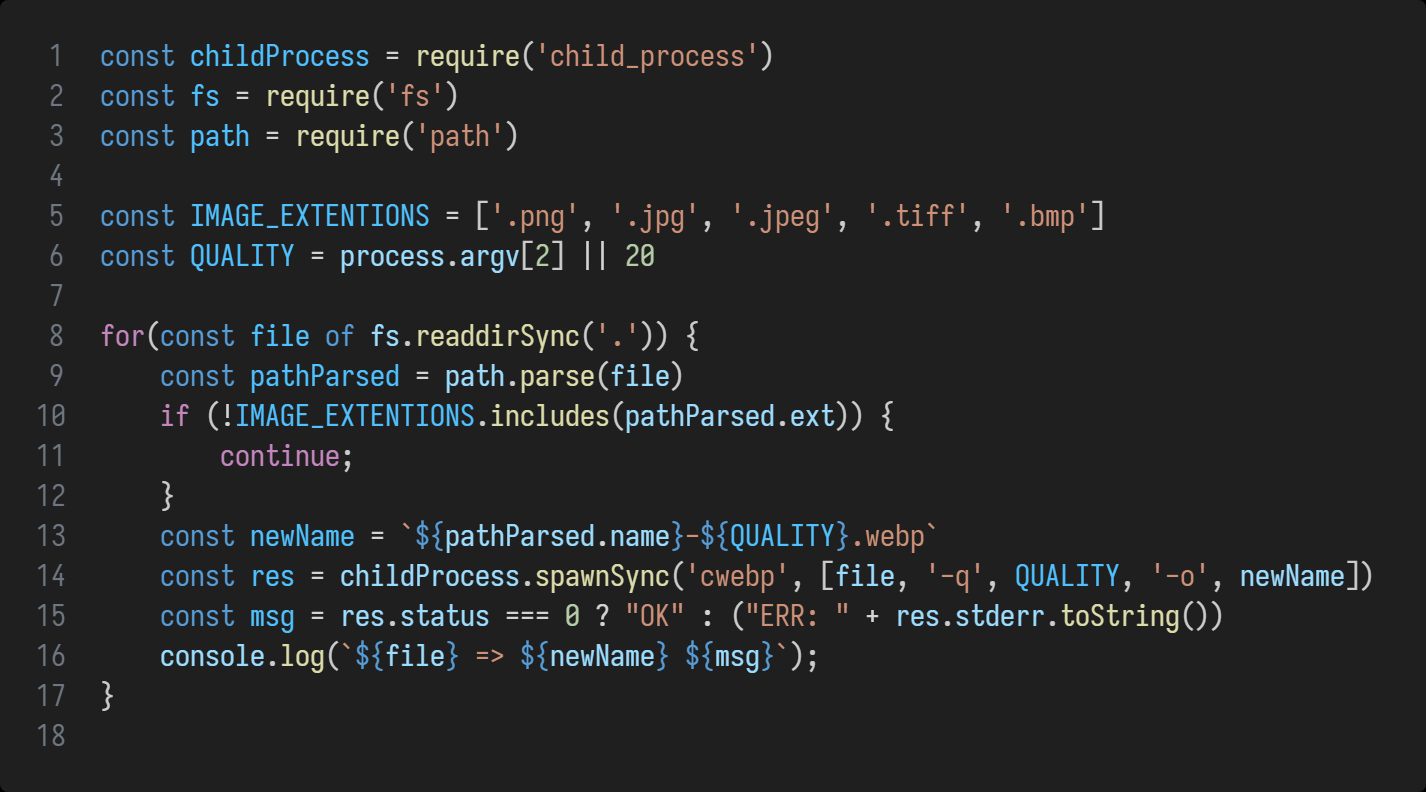
\includegraphics[width=\linewidth]{images/code_script_conv_webm.png}
  \caption{Skrypt konwertujący zdjęcia na format WebP}
  \label{fig:script-webp}
\end{figure}

Po uruchomieniu tego procesu w folderze ze zdjęciami, używając domyślnego parametru jakości równego 20, wygenerowane zostały nowe wersje wszystkich plików zdjęć na stronie. Finalny ich łączny rozmiar to $794.5$KB. W porównaniu do wcześniejszych $46.6$MB, jest to zmniejszenie o $98.3\%$, co jest wielką poprawą.

Możemy więc przetestować wpływ na wczytywanie witryny, przeprowadzając test WebPageTest'u.

\begin{figure}[H]
  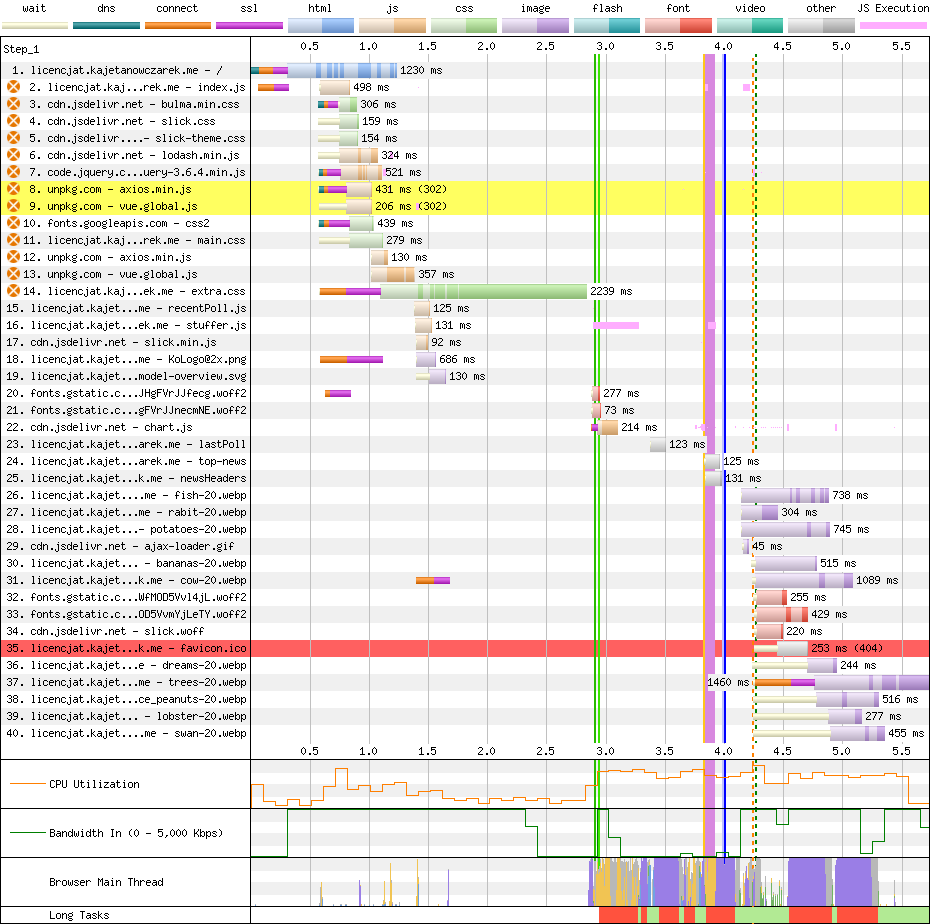
\includegraphics[width=\linewidth]{images/waterfall-after-webp.png}
  \caption{Wyniki testu po zmianie formatu zdjęć z PNG na WebP}
  \label{fig:waterfall-after-webp}
\end{figure}

Jak widać, zminiejszenie rozmiaru zdjęć o ponad $98\%$ odbiło się na czas wczytywania równie intensywnie, co wartość procentowa by sugerowała. Łączny czas wczytywania strony spadł z ponad $82$ sekund do $5.7$ sekundy. Niezmiennie, teraz, kiedy wykres nie jest zdominowany przez wczytywanie zdjęć na końcu procesu ładowania witryny, możemy zauważyć detale tego, co dzieje się w piewszych sekundach po nawigowaniu na naszą stonę.

\section{Analiza wczytywania 2}
Dzięki przeskalowaniu naszego wykresu, możemy ujrzeć dwa elementy, które wcześniej były zbytnio ściśnięte, by móc się im dobrze przyjżeć. Są nimi wcześniej wspomniane pionowe kreski oraz cieńkie elementy wierszy wykesu, repezentujące nawiązywanie połączeń i wykonywanie kodu JavaScript.

Pionowe znaczniki pokazują, kiedy odbywają się kluczowe momenty w procesie wczytywania witryny. Chronologicznie, pierwsze dwie zielone kreski oznaczają, kiedy przeglądarka rozpocznie proces generowania obrazu do wyświetlenia, oraz kiedy po raz pierwszy rezultaty renderowania strony zostaną pokazane użytkownikowi. 

Następna para, w kolorze pomarańczowym oraz fioletowym, przedstawia wydarzenia zakończenia wczytywania. Pomrańczowa kreska oznacza punkt zmiany stanu gotowości dokumentu na \verb|interactive|, co oznacza, że wszystkie dane głównego dokumentu HTML zostały już wczytane i przetworzone, ale podzasoby, jak pliki zdjęć, skyptów, stylów czy osadzone, inne dokumenty, mogą jeszcze się wczytywać\footnote{\url{https://html.spec.whatwg.org/multipage/dom.html\#current-document-readiness}}. Od tego momentu, strona jest w stanie reagować na wejścia użytkownika, jak używanie elementów formularzy, ale nie znaczy to, że całość interaktywnej funkcjonalności strony jest już gotowa, jedynie że możliwość użycia takich funkcji przez użytkownika może istnieć dla niektórych witryn. Fioletowy znacznik pokazuje, kiedy było obsługiwane zdarzenie \verb|DOMContentLoaded|, które jest uruchamiane w reakcji na zmianę stanu gotowości dokumentu. Te dwa wydarzenia powinny zawsze następować bezpośrednio po sobie, natomiast ich szerokość na wykesie oznacza, ile czasu zajeło przetwarzanie tych zmian przez nasłuchujący na nie kod.

Następna para znaczników (acz jeden z nich, jasnoniebieski, nie jest na wykresie dla tej strony pokazany\footnote{Ponieważ strona ta nie używa wydarzenia \texttt{load}, WebPageTest pomija jego znacznik na wykresie. Dla strony która go używa, pojawiłby się on natychmiastowo po ciemnoniebieskiej kresce.}) jest analogiczna do tych właśnie omówionych, ale stan gotowości dokumentu zmienia się na \texttt{complete}, a odpalone wydarzenie to \texttt{load}. Oznaczają one, że głowny dokument jak i jego podzasoby został w pełni wczytane i przetworzone. 

Kolejne dwa wskaźniki, tym razem przerywane, pokazują zmiany w wyglądzie naszej strony. Pomarańczowy pokazuje moment największej zmiany układu strony, kiedy to najwięcej elementów musiało zmienić swój układ i pozycję. Zielony za to, kiedy nastąpiła największa zmiana w obrazie wyświetlanym przez przeglądarke\footnote{Choć może się wydawać, że te dwa wydarzenia powinny być tym samym, nie koniecznie musi tak być. Przykładowo, strona może najpierw wczytać skórkę, jak tryb ciemny czy wysokiego kontrastu, powodując zmianę wartości pikseli na całym ekranie, a dopiero później wczytać samą treść, sprawiając, że przeglądarka musi ponownie obliczyć układ dokumentu.}. Zmiana przedstawiana przez zieloną kreskę jest nazywana powszechnie, w tym przez WebPageTest, Largest Contentful Paint, w skrócie \textbf{LCP}.

\begin{figure}[H]
  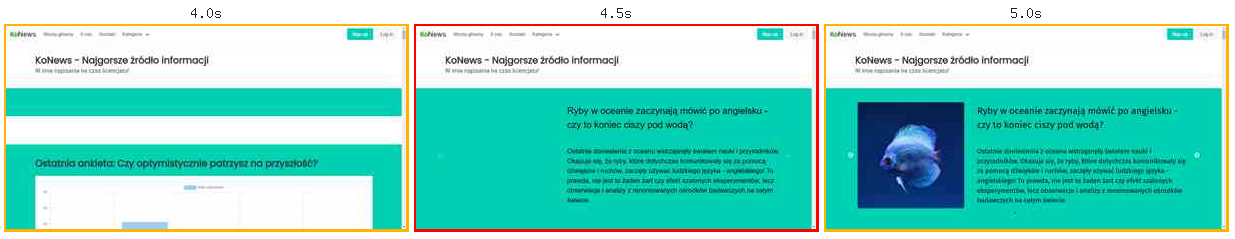
\includegraphics[width=\linewidth]{images/filmstrip.png}
  \caption{Zrzuty ekranu z wczytywania witryny, generowane przez WebPageTest. Wczytanie się zawartości tekstowej po $4.$ sekundzie zmieniło rozmiar nagłówka, przez co zawartość poniżej przesunęła się na stronie, co jest zanzaczone przez pomarańczową przerywaną linię. Wczytanie zawartości zdjęcia do sekundy $5.$ zmieniło wygląd strony, ale nie jej układ. }
  \label{fig:loading-layout-and-lcp}
\end{figure}

\selfnote{TODO Ponazywać te wydarzenia nazwami (LCP, TTI etc)}

Niektóre z tych metryk są skupione na technicznym aspekcie wczytywania strony, które obchodzą przede wszystkim nasz kod, oraz użytkowe, które są zauważalne przez użytkowników i wpływają na ich komfort używania witryny. Wymiana, która często pojawia się w dziedzinie optymalizacji, to wybór między szybszym wczytaniem całości strony, a przygotowaniem minimum używalnego dla użytkownika. Patrząc na czas do LCP, ponieważ nie cała stona jest wyświetlana na raz, można podjąć decyzję, aby poświęcić treści niżej na stronie, wczytująć je z mniejszym priorytetem, ale skracając czekanie na pokazanie się wstępnego wycinka zawartości, aby użytkownik mógł już mieć cokolwiek używalnego, w trakcie gdy reszta witryny dalej się wczytuje.

Na przykładowym projekcie, na którym prezentuję te techniki, zostały jeszcze okazje, by przyśpieszyć wczytywanie strony w spósób całkowity, ale po zastosowaniu tych zmian, skupię się miejscami na przyśpieszeniu wczytywania z perspektywy użytkownika, czyli kiedy strona wyświetla się i jest używalna, nawet jeżeli nie ma jeszcze pełni treści. Miejscami może to pogorszyć to czas do wczytania całości strony, ale poprawi subiektywne odczucie szybkości witryny, które starają się zmierzyć niektóre omówione heurystyki.

\section{Zmienianie rozmiarów zdjęć}

Prócz kompresji zdjęć, mamy jeszcze jedną taktykę na zmniejszenie ich kontrybucji w przesyle danych. Jest tym wybranie bardziej adekwatnych rozmiarów. Na ten moment, strona używa zdjęć w rozmiarze $2048\times2048$ pikseli, natomiast na wielu ekranach zdjęcia nie są nawet połowy tego rozmiaru.

Do zmiany rozmiaru zdjęć możemy użyć równieć narzędzia, którego użyliśmy do skompresowania zdjęć do formatu WebP, gdyż posiada on też opcje wycinania i zmiany rozmiru zdjęć. Zmodyfikowałem więc skrypt do konwersji, aby generował też obrazy o różnych, zadanych rozmiarach. 
Dzięki temu zmianie, skrypt generuje warianty tego samego zdjęcia, ale z innymi nazwami i rozmiarami.

\begin{figure}[H]
  \centering
  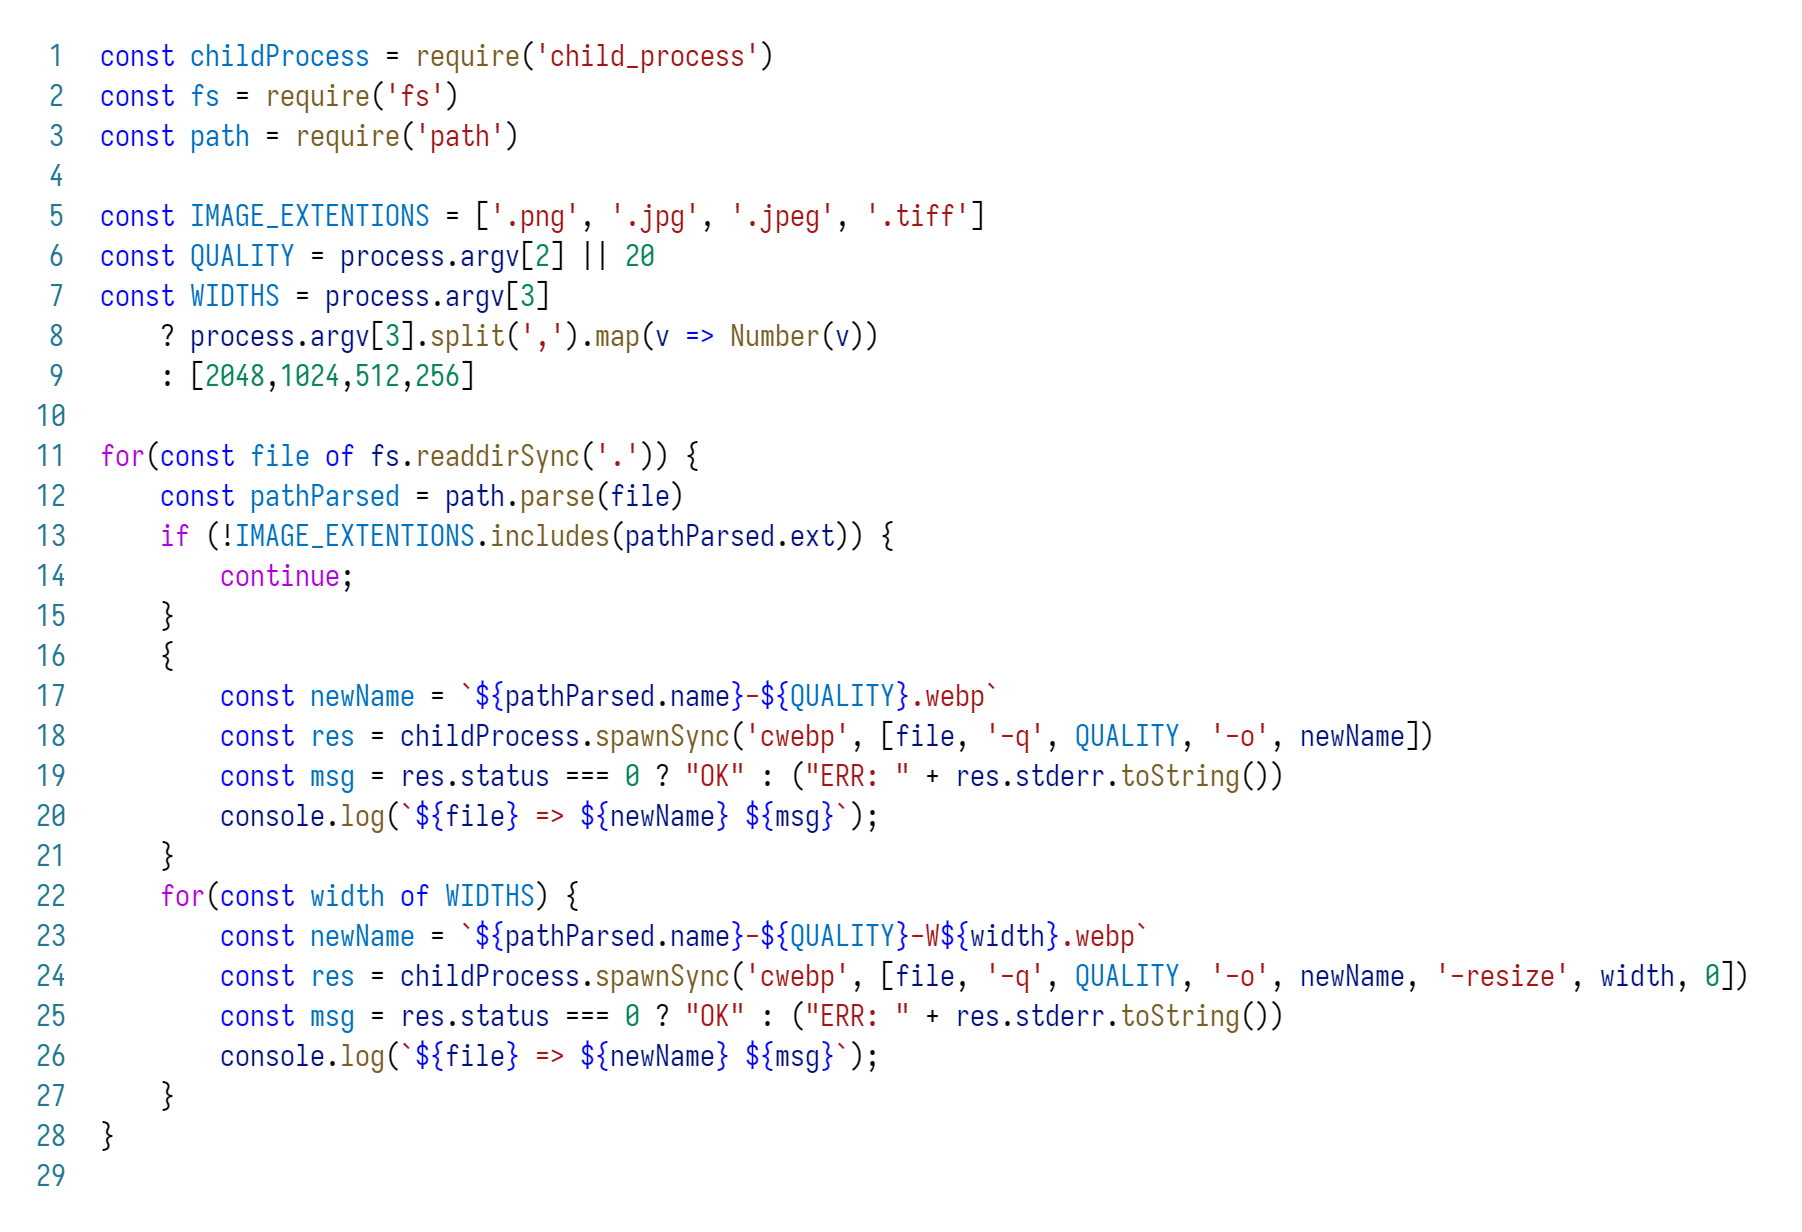
\includegraphics[width=\linewidth]{images/code_script_conv_format_and_size.png}
  \caption{Skrypt konwertujący format pliku, oraz generujący warianty w różnych rozmiarach}
  \label{fig:script-format-and-size}
\end{figure}

Mając takie pliki, możemy sprawić, że przeklądarka będzie wybierała optymalne rozmiarowo pliki dla danego urządzenia. Możemy to osiągnąć, modyfikując elementy \texttt{<img>}, aby używały atrybutów \texttt{srcset}\footnote{\url{https://html.spec.whatwg.org/multipage/images.html\#srcset-attribute}} oraz \texttt{sizes}, lub zamienić te elementy na elementy \texttt{picture}\footnote{\url{https://html.spec.whatwg.org/multipage/embedded-content.html\#the-picture-element}} oraz \texttt{source}. Tutaj użyję drugiej metody, ale obie polegają na wyrażeniu tego samego mechanizmu za pomocą różnej składni.

W połączeniu, elementy \texttt{picture} oraz \texttt{source} pozwalają wyświetlać w ramach jednego elementu pliki zdjęć wybrane na bazie CSS'owych kwerend \texttt{media}\footnote{\url{https://www.w3.org/TR/mediaqueries-4/}}. Możemy więc w ramach jednego elementu \texttt{picture} dostarczyć wiele różnych źródeł oraz warunki, aby były one użyte. Możemy więc przeanalizować, dla jakich układów naszej strony potrzebujemy jakiej rozdzielczości zdjęć, i stworzyć zestaw formatów, które sprawią, że do klienta będzie przesyłane nie więcej danych obrazów niż potrzeba.

Dla przykładowego projektu to, jakiej chcemy rozdzielczości nie jest tak proste. Jak widać na rys. \ref{fig:frontpage-articles}, na szerokim, komputerowym monitorze część naszych zdjęc jest wyświetlane w układzie z trzema kolumnami. Gdy jednak przejdziemy na ekran o wiele węższy, na przykłąd komórkowy, kolumny znikają, a karta artykułu, w tym zdjęcie, zajmuje całą szerokość ekranu. Przez to zachowanie, w miarę zmniejszania się ekranu wymagana rozdzielczość zdjęć maleje, ale w pewnym momencie (kiedy wyłącza się układ kolumnowy) rośnie.

\begin{figure}[H]
  \centering
  
\includegraphics[width=\linewidth/\real{3.5}]{images/screenshot-iphone11.png}
  \caption{Układ witryny dla ekranów mobilnych (rozmiar ekranu iPhone 11)}
  \label{fig:screenshot-iphone11}
\end{figure}

Jeszcze jednym elementem układu jest to, że na bardzo szerokich monitorach zawartość strony jest centrowana, zostawiając przestrzeń po bokach. Oznacza to, że od pewnej szerokości ekranu w górę, zdjęcia będą takiego samego rozmiaru. 

\begin{figure}[H]
  
\includegraphics[width=\linewidth]{images/screenshot-very-wide.png}
  \caption{Układ witryny dla bardzo szerokich ekranów}
  \label{fig:screenshot-verywide}
\end{figure}


Wiedząć, przy użyciu jakiej technologii zbudowana zostałą ta strona (framework CSS \texttt{Bulma}), oraz że nie były modyfikowane jej ustawienia, wiem również, że tą maksymalną szerokością ekranu jest $1408$ pikseli\footnote{\url{https://web.archive.org/web/20230518134357/https://bulma.io/documentation/layout/container/}}, przy którym centrowana treść dostaje szerokość $1344$ pikseli. W podobny sposób mogę sprawdzić, że układ kolumnowy wyłącza się na ekranach mniejszych niż $768$ pikseli\footnote{\url{https://web.archive.org/web/20230512141342/https://bulma.io/documentation/overview/responsiveness/}}.

Więdząc, jaki jest kod naszej witryny, możemy policzyć, ile dokładnie miejsca zajmie dane zdjęcie przy konkretnej szerokości ekranu. Można też użyć skryptów lub narzędzi developera, aby zmierzyć szerokości elementu wyświetlanego przez przeglądarkę.

\begin{figure}[H]
  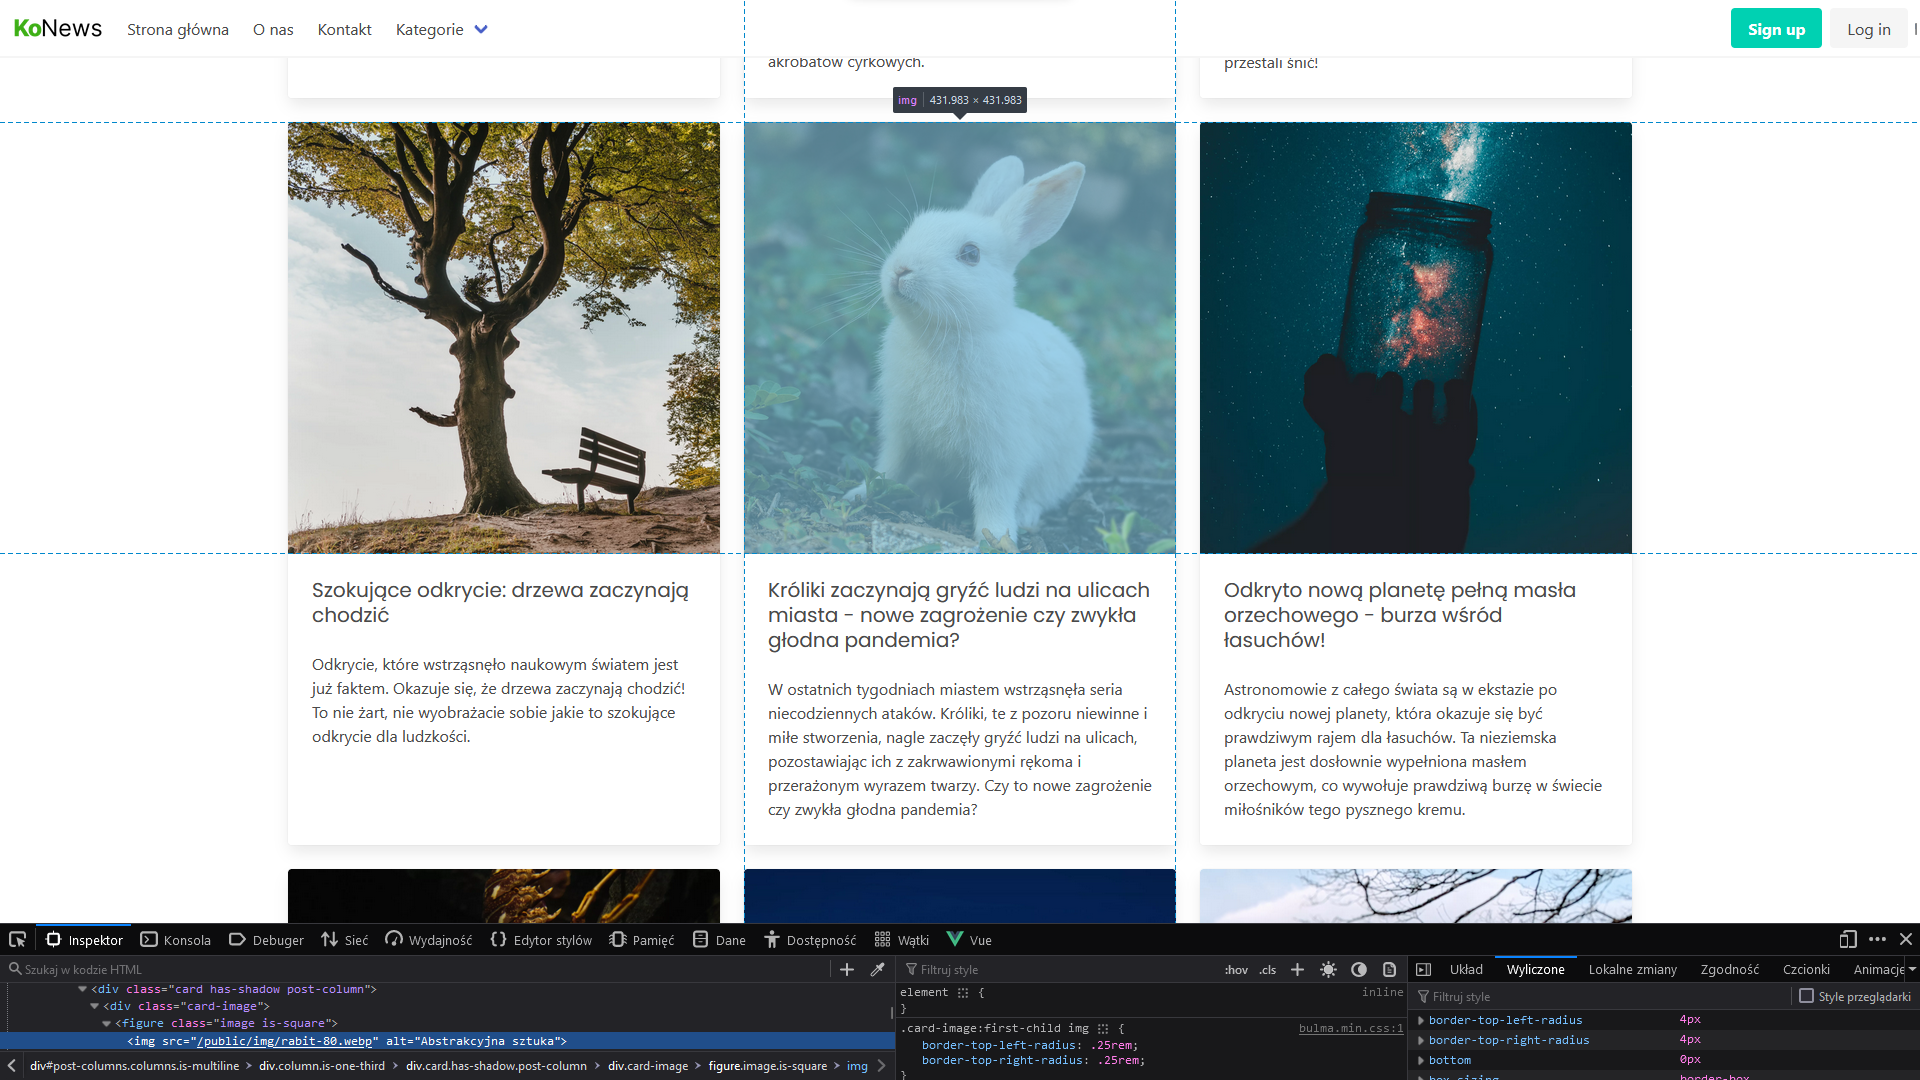
\includegraphics[width=\linewidth]{images/screenshot-devtools-1080width.png}
  \caption{Mierzenie rozmiaru zdjęcia za pomocą narzędzi developera. Tutaj, dla ekranu $1920\times1080$, zdjęcie jest kwadratem o boku ledwo co poniżej $432$ pikseli.}
  \label{fig:screenshot-measuring}
\end{figure}

Możemy więc takto przygotować pomiary dla kluczowych rozmiarów ekranu:

\begin{center}
  \begin{tabular}{|c|c|}
    \hline
    Szerokość ekranu (w pikselach) & Rozmiar zdjęcia (w pikselach) \\
    \hline
    $2560$ (Quad HD) & $432$ \\
    $1920$ (Full HD) & $432$ \\
    $1366$ & $368$ \\
    $1280$ (HD) & $368$ \\
    $1023$ (największy rozmiar tabletowy) & $309$ \\
    $770$ (najmniejszy niemobilny) & $225$ \\
    $769$ (mobilne wg Bulmy) & $720$ \\
    $640$ (SD) & $592$ \\
    $500$ & $452$ \\
    $320$ (iPhone 3) & $272$ \\
    $300$ & $252$ \\
    $200$ & $252$ \\
    \hline
  \end{tabular}
\end{center}

Jak widać, przez wyłączenie się systemu kolumn na ekranach moblinych, zdjęcia na węższych ekranach są większe, niż na dowolnie dużych. Dla dużych desktopowych rozdzielczości, Bulma przeskakuje między rozmiarami $432$ dla Full HD i $368$ dla zwykłego HD pikseli (aczkolwiek jest niewielkie okno rozmiarów ekranu, gdzie pomiędzy tymi dwoma rozdzielczościami zdjęcia mają inne, deliktanie mniejsze od $432$ rozmiary). Najmniejsze zdjęcie, jakie wyświetli się na niemobilnym ekranie ma bok $225$ pikseli, ale przy delikatnie mniejszym ekranie rozmiar zdjęcia wzrośnie do największego, jaki kiedykolwiek się wyświetli, czyli $720$ pikseli wysokości i szerokości. W formacie mobilnym zdjęcia maleją w równym tempie co ekran, będąc o $48$ pikseli mniejsze niż jego szerokość, aż do minimum $252$ pikseli.

Możemy więc znaleźć zestaw rozmiarów, które obsłuża potrzebne nam zakresy rozmiarów ekranu. Moglibyśmy generować niezliczone różne rozdzielczości, ale na potrzeby tej strony wystarczający wydaje się zestaw:

\begin{itemize}
  \item $720$ pikseli, dla dużych telefonów,
  \item $432$ piksele, dla dużych komputerów i średnich telefonów,
  \item $368$ pikseli, dla mniejszych komputerów i małych telefonów.
\end{itemize}
 
Po wygenerowaniu naszych obrazów za pomocą skryptu, musimy też dodać obsługę zmiennych rozmiarów w kodzie witryny. Do generowania elementów artykułów na stronie, używany jest framework Vue. Możemy więc zmienić wzorzec, który jest używany przez kod, aby dynamicznie wygenerować treść.

\begin{figure}[H]
  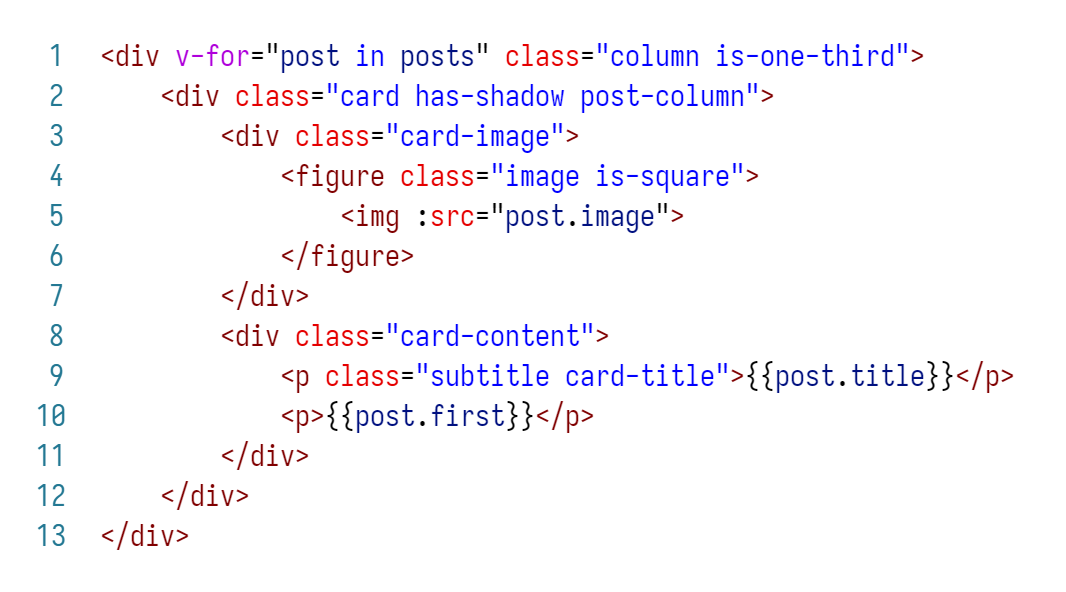
\includegraphics[width=\linewidth]{images/code-vue-image-card-old.png}
  \caption{Wzorzec Vue używany do generowania kart z artykułami}
  \label{fig:code-vue-template-articles-old}
\end{figure}

W środku tego wzorca, znajdujemy element \texttt{<img>}, którego właściwość \texttt{src} jest dynamicznie ustawiana przez Vue na konkretną, zadaną wartość (Znak \texttt{:} jest używany w Vue do oznaczania właściwości dynamicznych. Tutaj, jest to pole \texttt{image} na obiekcie \texttt{post}.)

Musimy też stworzyć mechanizm, aby wybierać, które zdjęcie ma być wysłane z serwera. W moim przypadku zdecydowałem, żeby serwer wysyłał adres URL zdjęcia z tekstem WIDTH w miejscu, w które należy wstawić żadaną szerokość obrazu. Kod na stronie będzie musiał więc podmieniać ten ciąg na żądaną szerokość w pikselach.

Możemy więc obwinąć element \texttt{<img>} w element \texttt{<picture>}. W takiej konfiguracji, jeżeli mechanizm wybierania lepiej dopasowanych treści nie wybierze żadnego zasobu, to element \texttt{<img>} zostanie użyty jako domyślna wartość.

Możemy więc stworzyć następujący wzorzec:

\begin{figure}[H]
  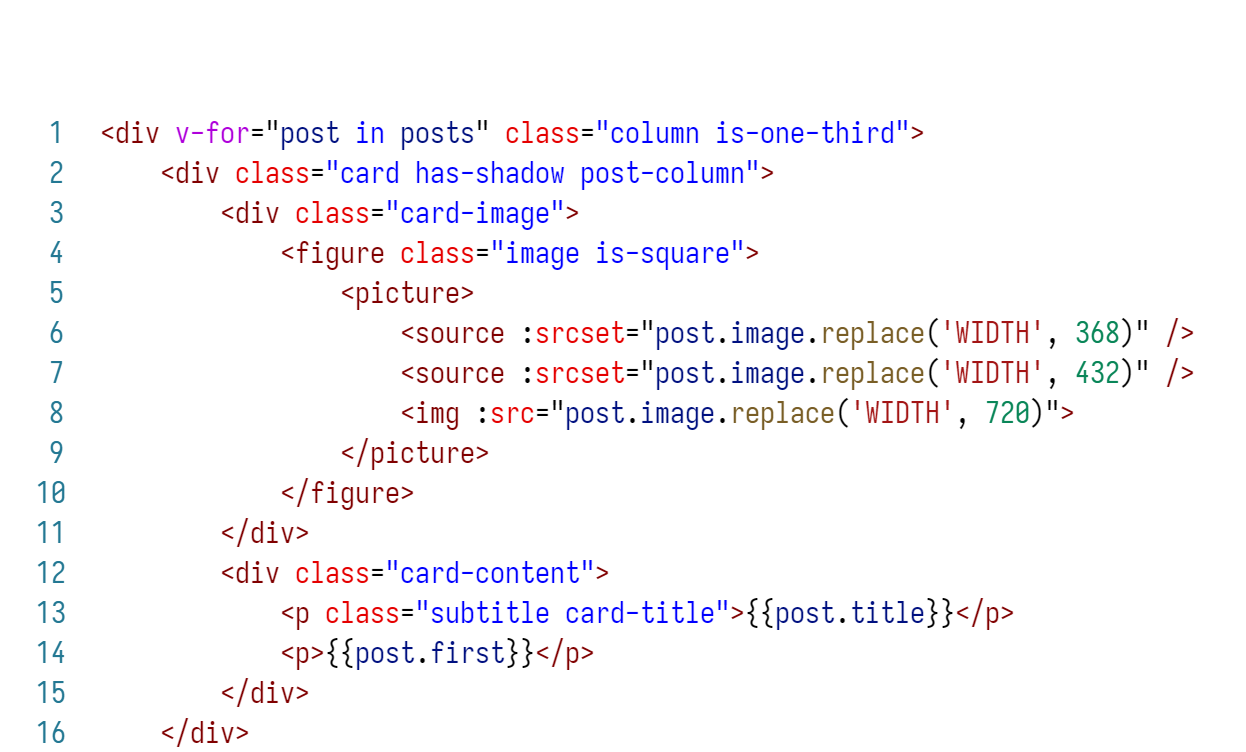
\includegraphics[width=\linewidth]{images/code-vue-image-card-mid.png}
  \caption{Wzorzec częściowo zmodyfikowany, aby używać resposnywnych obrazów}
  \label{fig:code-vue-template-articles-mid}
\end{figure}

Niestety, to jeszcze nie koniec zmian, które musimy wprowadzić. Gdybyśmy otworzyli teraz naszą witrynę, zobaczylibyśmy wiele rozmytych zdjęć. Wynika to z tego, że nie podaliśmy kwerend \texttt{media}, które ustalałyby, które ze źródeł wybrać do wyświetlenia. Musimy więc wybrać, w jakim zakesie szerokości ekranów mają być użyte dane obrazy. Patrząc na nasze poprzednie analizy, możemy stwierdzić, że:

\begin{itemize}
  \item Zdjęcia o szerokości $368$ pikseli powinny być użyte na ekranach szerszych niż $769$, ale węższych lub równych $1366$ pikseli, oraz na węższych niż $416$ pikseli,
  \item Zdjęcia o szerokości $432$ pikseli powinny być użyte na ekranach o szerokości ponad $1366$ pikseli, oraz na szerszych niż $416$, ale węższych niż $480$ pikseli
  \item Zdjęcia o szerokości $720$ pikseli powinny być użwyane na ekranach węższych lub równych $769$, ale szerszych niż $480$ pikseli
\end{itemize}

Rozmiary są do tego testowane od pierwszego w kodzie do ostatniego, wybierając pierwszy, na który kwerenda \texttt{media} zezwala. Ponieważ rozmiar $720\text{px}$ traktujemy jako domyślną, oraz ponieważ jego przedział jest tam, gdzie nie jest pozostałych dwóch, możemy zostawić element \texttt{<img>}, który jest za ten rozmiar odpowiedzialny, zostawić jaki jest.

%\selfnote{Napisać o tym, że ten mechanizm działa na bazie szerokości}

Rozmiar $368\text{px}$ jest preferowany dla szerokości z zakresu $\rinterval{0}{416\text{px}} \cup \linterval{769\text{px}}{1366\text{px}}$. Żeby przekonwertować zakres zamknięty $\interval{a}{b}$ na kwerendę \texttt{media}, odpowiadający kod to \texttt{(min-width: a) and (max-width: b)}. Niestety nie ma sposobu, żeby przekonwertować zakes otwarty, musimy więc wziąc zakes zamknięty z o jeden większą lub mniejszą żądaną granicą przedziału szerokości. Jeżeli dolna granica to zero, oraz kiedy górna jest w nieskończoności, możemy pominąć ich część kodu. Aby wyrazić w kodzie, że dane źródło jest preferowane dla więcej niż jednej kwerendy, tutaj reprezentujących zakresy szerokości, możemy postawić kody tych kwerend po przecinku.
Tak więc kwerenda \texttt{media}, która wyśwetli zdjęcie o szerokości $368\text{px}$, zgodnie z wyżej opisanymi wymaganiami, to:
\begin{verbatim}
  (max-width: 416px), (min-width: 770px) and (max-width: 1366px)
\end{verbatim}
Podobnie możemy napisać kwerendę dla zdjęć o szerokości $432\text{px}$:
\begin{verbatim}
  (min-width: 417px) and (max-width: 480px), (min-width: 1367px)
\end{verbatim}
Dla pozostałych przypadków obsługuje nas domyślny przypadek, więc mamy już wszystkie elementy, żeby w pełni zaimplementować responsywne dopasowywanie rozmiaru zdjęć. Łącząc wszystko, co potrzebne, dostajemy kod:

\begin{figure}[H]
  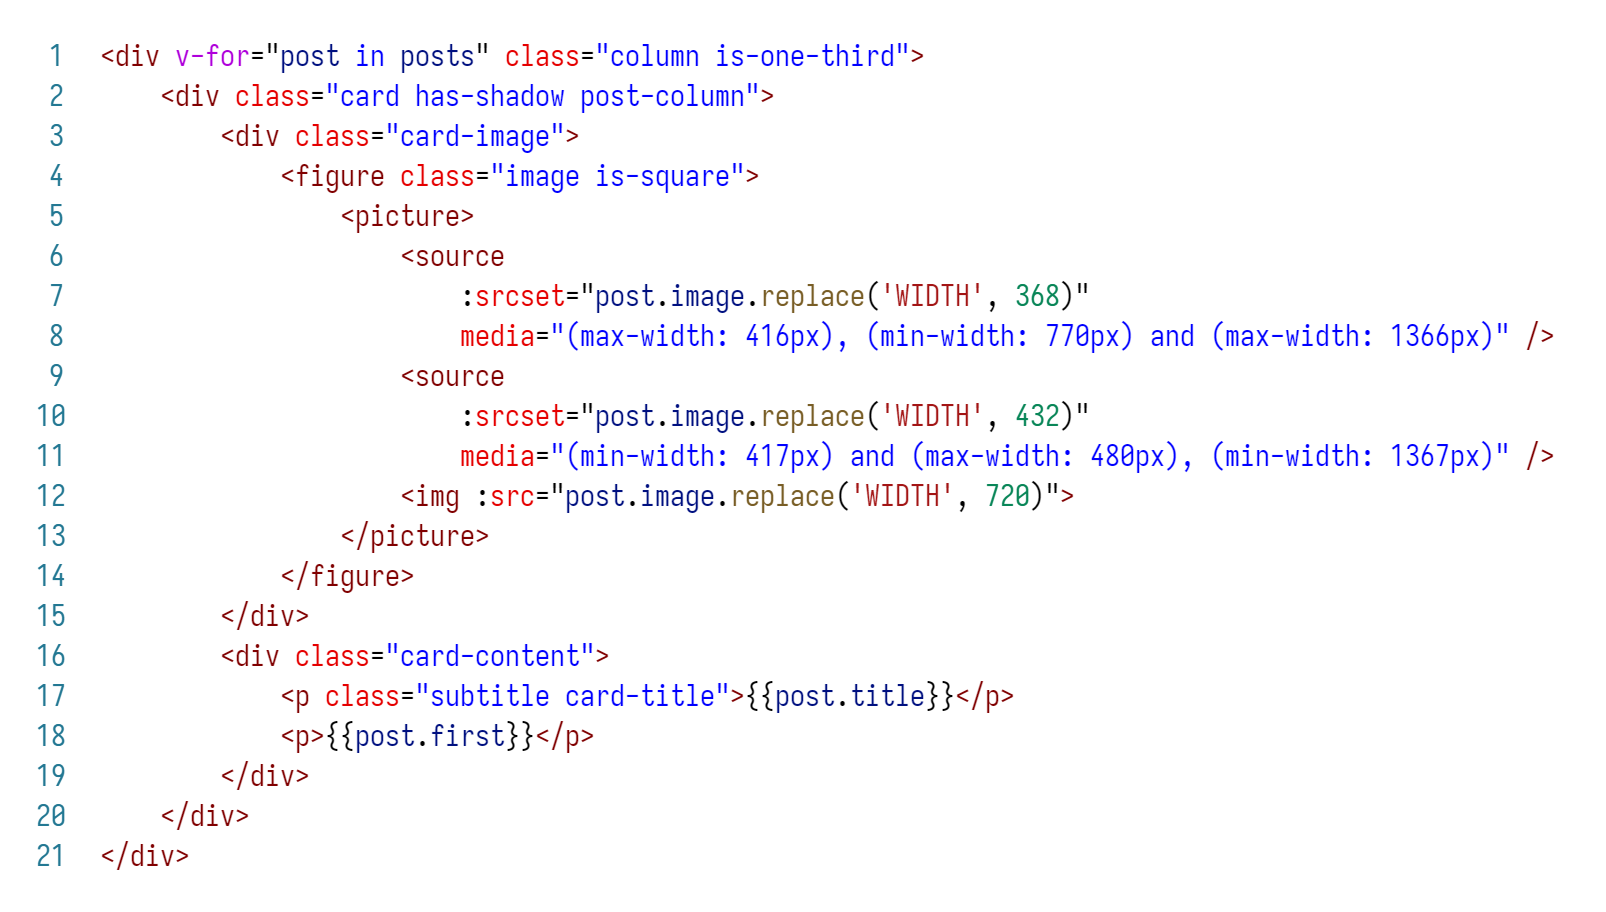
\includegraphics[width=\linewidth]{images/code-vue-image-card-done.png}
  \caption{Zakończony wzorzec, który wybiera zdjęcia o optymalnie małym rozmiarze, aby przesłać jak najmniej danych}
  \label{fig:code-vue-template-articles-done}
\end{figure}

Niefortunnym aspektem tej optymalizacji jest to, że będzie ona przynosiła nieco inne efekty dla różnych konfiguracji tego samego sprzętu. Choć wiele razy było opisywane, że mechanizm korzysta z szerokości ekranu, aby ustalić, jakie źródło dla obrazu wybrać, tak jest to prawdą tylko, jeżeli okno przeglądarki zajmuje całą szerokość ekranu. Jeżeli zajmuje ono tylko jakąś część ekranu, to tylko ta część jest traktowana w ramach mechanizmu wyboru.

Testując nasze zmiany przy użyciu WebPageTest'u, dostajemy następujące wyniki:

\begin{figure}[H]
  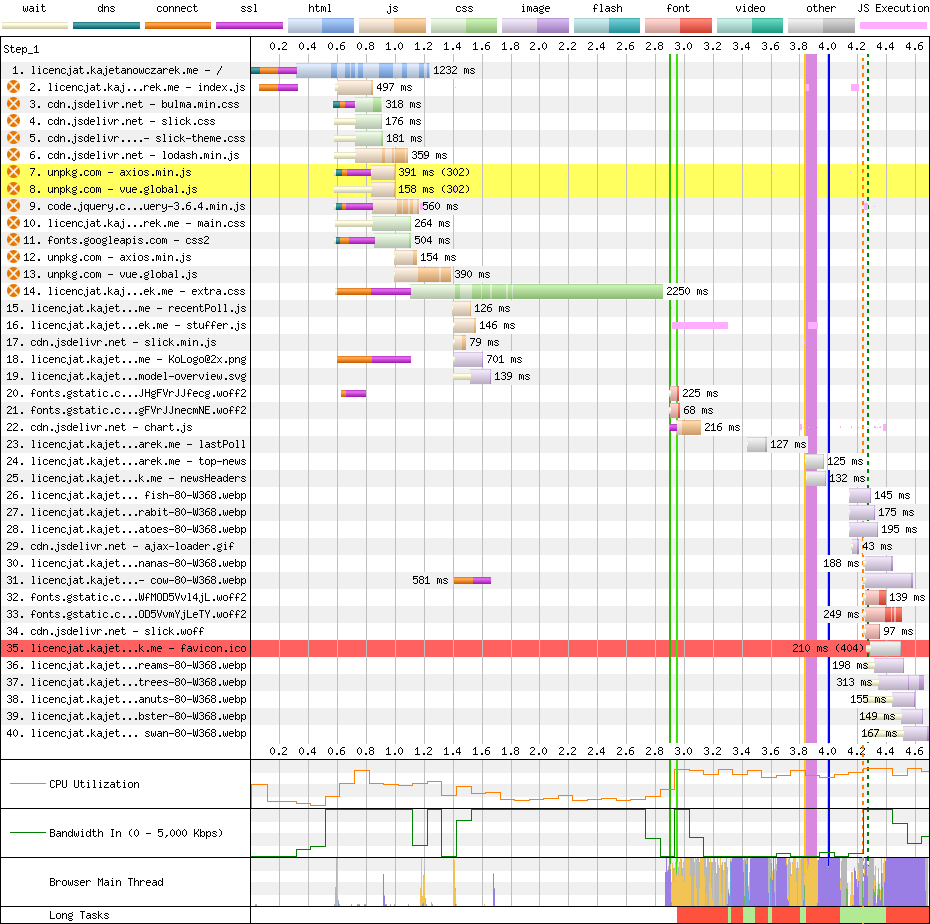
\includegraphics[width=\linewidth]{images/waterfall-after-sizing.png}
  \caption{Wyniki testów bo wdrożeniu responsywnego wyboru zdjęć}
  \label{fig:waterfall-after-sizing}
\end{figure}

Porównując z poprzednim testem, łączny czas wczytywania się strony spadł z $5.7\text{sek}$ do $4.7\text{sek}$, więc udało nam się odzyskać sekundę czasu przy każdym wczytaniu naszej strony. Niestety, ponieważ zdjęcia te nie blokowały pierwszego wyświetlenia, ani nie powodowały, że użytkownik czekał na ich wczytanie, aby móc korzystać z interaktywności, nie poprawiły się pozostałę metryki. Niezmiennie, jest to poprawa czasu, jak i oszczędności kosztu transferu danych, a choć czas do zobaczenia przez użytkownika jakieś treści na naszej witrynie nie jest mniejszy, tak mniej czasu będzie spędzone na patrzeniu się na niewczytane lub częściowo wczytane zdjęcia, więc poprawiliśmy używalność podczas wczytywania naszej witryny.

Alternatywnym sposobem, aby zrealizować podobny efekt optymalizacji, byłoby najpiew wczytanie zasobów w niskiej rozdzielczości, a kiedy strona będzie już w pełni wczytana, zacząć zamieniać ja wyższorozdzielczościowe wersje. Nie omówię tutaj, jak zastosować tą technikę, gdyż ma ona ograniczone wsparcie wśród standardów webowych, więc całość implementacji jest po stronie twórcy witryny. Zbliżona technika do tej będzie zaprezentowana później, acz w kontekście czcionek.


\section{Użycie kompresji bezstratnej}

Póki co użyliśmy kompresji zdjęć, aby znacznie zmniejszyć rozmiar plików witryny. Była to kompresja stratna, gdyż nie wszystke detale oryginalnych zdjęć zachowały się przez cały proces, lecz dalej zawarte jest ich wystarczająco dużo, aby obrazy były czytelne. Takiego rodzju kompresji nie możemy zastosować do kodu naszej strony, gdyż każdy ich detal jest kluczowy dla poprawnego funkcjonowania witryny. Możemy jednak użyć kompresji bezstratnej.

Jest wiele różnych algorytmów na bezstratną kompresję danych, ale w ramach tego projektu użyjemy formatu plików \texttt{gzip}, który używa  algorytmu kompresji \texttt{DEFLATE}\footnote{\url{https://www.ietf.org/rfc/rfc1952.txt}, strona 5}.

Algorytm \texttt{DEFLATE} kompresuje dane w dwóch krokach. Pierwszy, to bazowany na algorytmie \texttt{Lempel-Ziv77} mechanizm usuwania powtórzeń, który zastępuje niepierwsze wystąpienia sekwencji bajtów odniesieniami do ich poprzednich wystąpień. Drugi, to rozszerzenie kodowania Huffmana, które poświęca prostotę przetwarzania w modelu "1 bajt, kodujący jeden znak\footnote{Kodowania, gdzie 1 bit to jeden znak są popularne, acz definitywnie nie są jedynym systemem. \texttt{ASCII} koduje jeden znak w $7$miu bitach, natomiast \texttt{Unicode} korzysta ze zmiennej ilości bajtów do przedstwienia jednego symbolu.}, w równych odstępach" na rzecz systemu korzystającego ze zmienniej długości bitowej znaku, nadając najpowszechniej występującym znakom krótsze reprezentacje. Rozszerzenie użyte w algorytnie \texttt{DEFLATE} polega na dodaniu do drzewa Huffmana znaków nie reprezentujących danych, a rodzaje odniesień wygenerowanych przez pierwszy krok.

Ponieważ algorytmy te są bardzo powszechnie używane w internecie, obsługa ich w bardzo wielu przypadkach powinna być bardzo prosta. Serwer, z którego korzystam do wystawiania testowej witryny, korzysta z programu \texttt{nginx} jako serwer. Żeby więc włączyć obsługę kompersji \texttt{gzip}, wystarczy zmodyfikować plik konfiguracji tego serwera, dodając dyrektywy \texttt{gzip on;} oraz ustawiając rodzaje odpowiedzi, które powinny być kompresowane. Mając więc plik konfiguracji wyglądający następująco:
\begin{figure}[H]
  \centering
  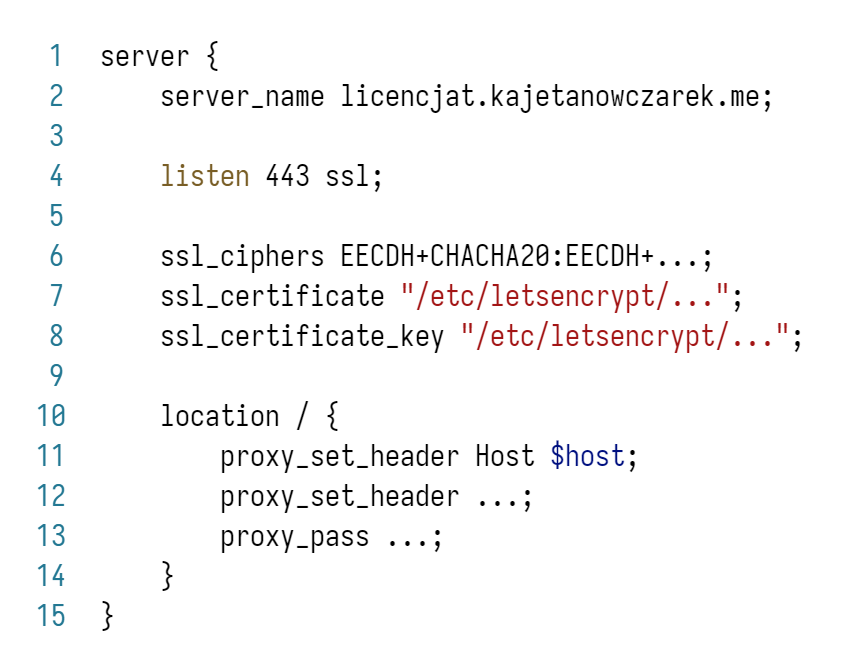
\includegraphics[width=\linewidth/\real{1.55}]{images/code-nginx-conf-trunc-nogzip.png}
  \caption{Plik konfiguracji nginx, używany przez prawdziwy serwer, z którego pochodzą wyniki pomiarów, z pominientymi danymi zbędnymi do tego tematu.}
  \label{fig:nginx-before-gzip}
\end{figure}
możemy dodać obsługę kompresowania do formatu \texttt{gzip} naszych plików \texttt{HTML}, \texttt{CSS} i \texttt{JavaScript}, zmieniając zawartość tego pliku na:
\begin{figure}[H]
  \centering
  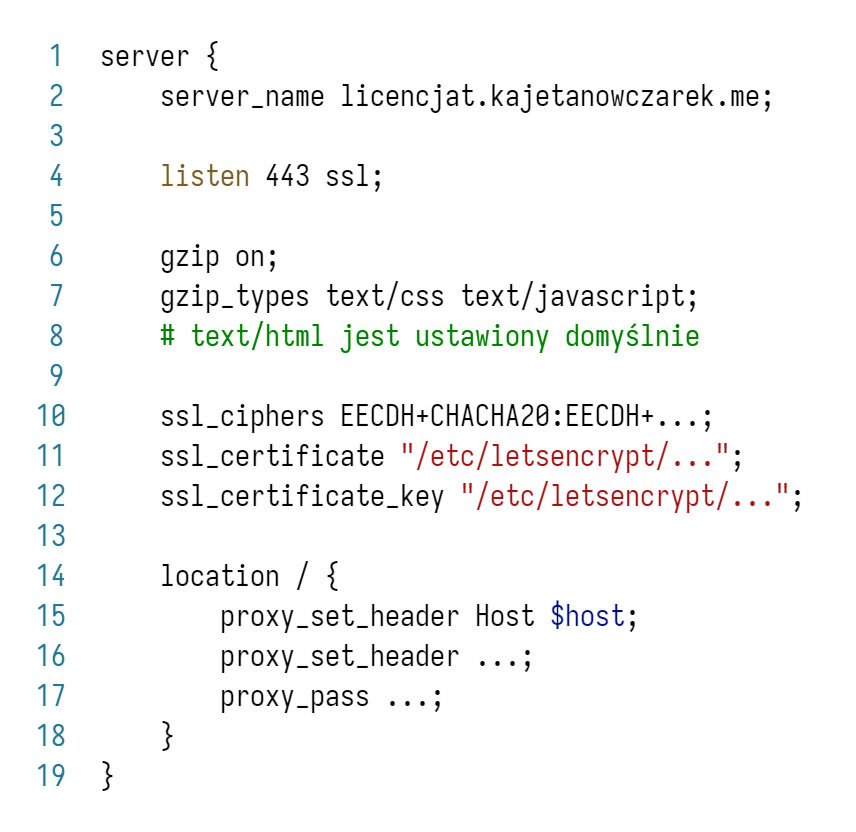
\includegraphics[width=\linewidth/\real{1.55}]{images/code-nginx-conf-trunc-gzip.png}
  \caption{Zmodyfikowany plik konfiguracji nginx, uruchamiający kompresję \texttt{gzip} odpowiedzi o formacie \texttt{MIME} \texttt{text/html}, \texttt{text/css} i \texttt{text/javascript}.}
  \label{fig:nginx-after-gzip}
\end{figure}

Po zastosowaniu tej zmiany, ponownym uruchomieniu \texttt{nginx} i ponownym przetestowaniu, otrzymujemy następujące wyniki:
\begin{figure}[H]
  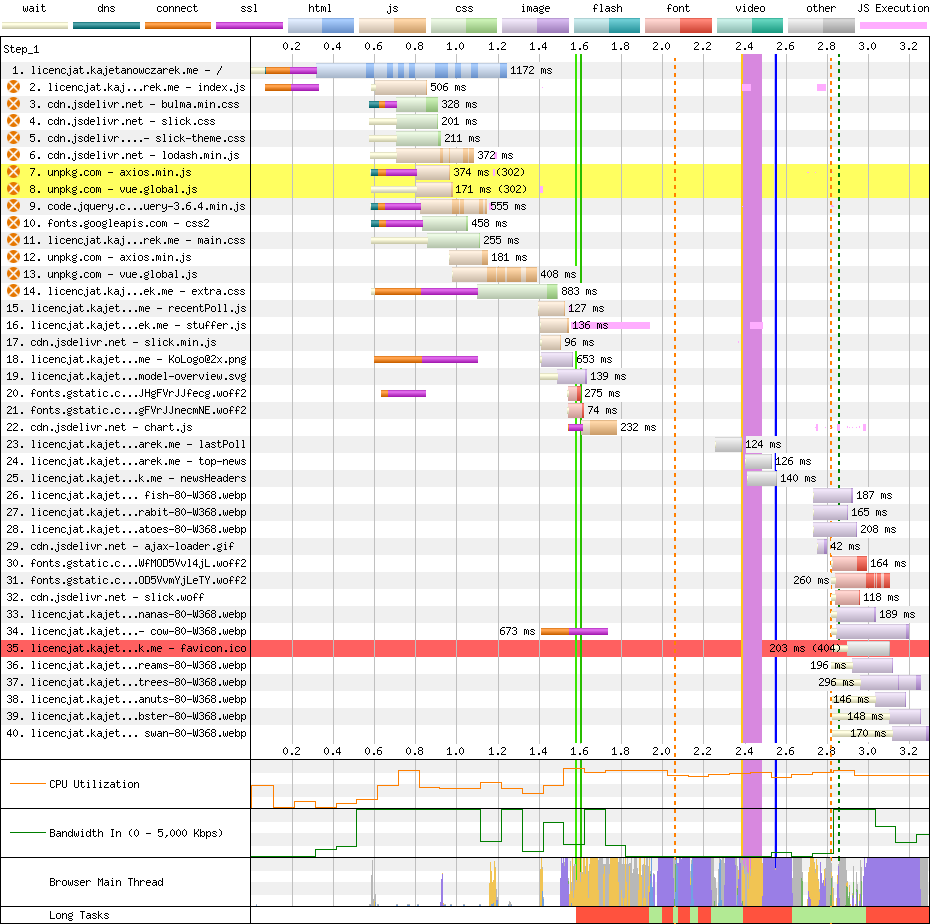
\includegraphics[width=\linewidth]{images/waterfall-after-gzip.png}
  \caption{Wyniki testów WebPageTest po uruchomieniu kompresji \texttt{gzip}}
  \label{fig:waterfall-after-gzip}
\end{figure}

Jak możemy zauważyć, największym źródłem poprawy czasu wczytywania jest znaczne przyśpieszenie wczytywania pliku \texttt{extra.css}. Prócz tego, poprawy są bardzo ograniczone, co wynika z tego, że duża część zasobów tego typu nie była wysyłana przez nas serwer, a przez serwery usług \texttt{jsdelivr} oraz \texttt{unpkg}, które hostują używane przez strony biblioteki. Ponieważ połączenie nie jest nawiązywane z naszym serwerem, włączenie na nim kompresji nie wpływa na to, jak zostaną wykonane te połączenia.




\section{Sprytniejsze stylowanie}

Kontynuując poprawianie naszej witryny, możemy zwrócić naszą uwagę do zasobów \texttt{CSS}. Choć po skompresowaniu, plik \texttt{extra.css} nie zabiera tak wiele czasu jak wcześniej, tak jest on drugim najdłużej wczytywanym plikiem, zaraz po głównym dokumencie. Ponieważ pliki \texttt{CSS}, które opisują, jak elementy naszej witryny mają wyglądać na ekranie, są zasobami blokującymi wyświetlanie\footnote{\url{https://html.spec.whatwg.org/\#render-blocking-mechanism}}, które dopóki są wczytywane, uniemożliwiają wyświetlenie zawartości strony. Przyśpieszając więc czas ich wczytania, sprawimy, że na witrynie treści zostaną przedstawione użytkownikowi wcześniej.

Szukając okazji do uzyskania wcześniejszego wczytania, rozważmy zmniejszenie rozmiaru plików \texttt{CSS}. Przyglądając się waterfallowi z rysunku \ref{fig:waterfall-after-gzip}, możemy zauważyć, że większość zielonych prostokątów, oznaczających zapytania pobierające pliki \texttt{CSS}, jest w swojej bladej wariacji kolorowej. Oznacza to, że niewiele czasu zostało poświęcone na pobieranie, a wiele na czekanie na dane. Dodatkowo, cieńsze białę kreski przed zielonymi prostokątami pokazują, że zapytania te nie były w stanie przejść natychmiastowo do gotowości do pobierania, a musiały poczekać na skończenie innych aktywności. 

Pomimo tego, że większość czasu poświęconego na arkusze stylów był spędzony na czekaniu, możemy zauważyć dwa bloki bardziej nasyconego zielonego. Pierwszy jest częścią pobierania pliku \texttt{bulma.min.css}, który zawaiera użwaną przez projekt bibliotekę, zbitą w jeden plik zawierający całość funkcji biblioteki. Drugi za to jest powiązany z plikiem \texttt{extra.css}, który jest częścią niebibliotecznego kodu projektu.

Plik \texttt{extra.css} przedstwia bibliotekę CSS'ową, która zawiera wiele tzw. utility classes, klas obiektów pozwalających na dostosowanie wyglądu elementów wyłącznie z poziomu kodu HTML, poprzez użycie wielu klas zawierających w swojej nazwie żądany parametr. W przyadku tego projektu, używane są dwa rodzaje takich klas\footnote{Choć te dwa przypadki są definitywnie przesadzone w skali ilości opcji parametrów, mają one przestawiać odpowiednik wielu mniejszych klas. Ignorując nieco detali związanych z kompresją, można zająć podobną ilość danych, używając wielu utility class o mniejszej liczbie opcji na ich parametry.} - trójka klass \texttt{luma-\#}, \texttt{luma-bg-\#} oraz \texttt{fix-text}, oraz element siatki, otrzymujący dwa parametry w dwóch klasach, \texttt{row-\#} oraz \texttt{col-\#}.

Klasa \texttt{luma-\#}, gdzie \texttt{\#} to liczba od $0$ do $255$, gdy dodana do elementu sprawia, że zawarty tekst przyjmuje kolor w odcieni szarości zależny od liczby \texttt{\#}, poprzez nadanie mu koloru z przestrzenii \texttt{RGB}, z wartościami wszystkich kanałów ustawionymi na \texttt{\#}. Klasa \texttt{luma-bg-\#} wybiera ten sam kolor, co \texttt{luma-\#}, jednak ustawia go na kolor tła, a nie tekstu. Klasa \texttt{fix-text}, kiedy jest ustawiona na elemencie z \texttt{luma-bg-\#}, lub kiedy element dziedziczny takowego ją posiada, ustawia tekst na kontrastujący - biały dla $\texttt{\#} < 127$, czarny dla $\texttt{\#} \geq 127$.

\begin{figure}[H]
  \centering
  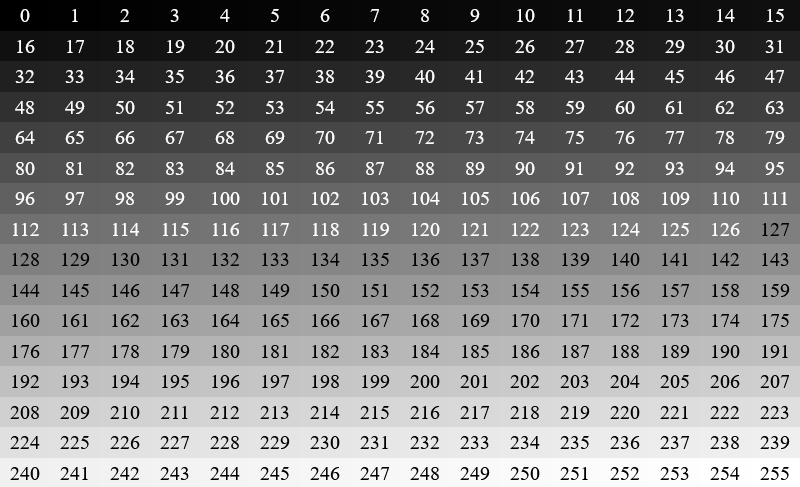
\includegraphics[width=\linewidth]{images/ui-luma-grid.png}
  \caption{Efekt, który chcemy osiągnąć}
  \label{fig:ui-luma-grid}
\end{figure}

Sposóby na osiągnięcie takiej funkcjonalności dla wielu przeglądarek przed 2016\footnote{Rok wzięty z \url{https://caniuse.com/css-variables} - wcześniej tylko Firefox implementował zmienne \texttt{CSS}} polegały na wielokrotnej duplikacji kodu, poprzez rzeczywiste stworzenie klasy dla każdej rządanej opcji parametru.

\begin{figure}[H]
  \centering
  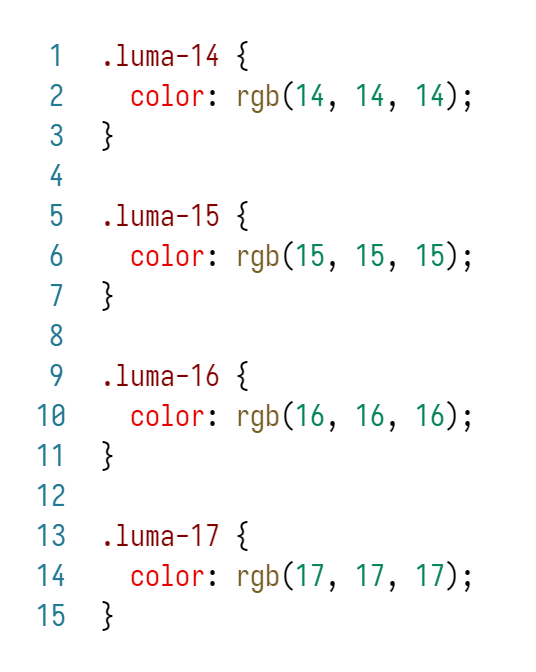
\includegraphics[width=\linewidth/\real{2.5}]{images/code-css-luma.png}
  \caption{Wycinek pliku \texttt{extra.css}, definiujący parę wariantów jednek z klas. Podobny kod jest powtórzony wiele razy w reszcie pliku.}
  \label{fig:css-css-luma}
\end{figure}

Elementem, który ratuje delikatnie ten kod, to jego podatność na zmniejszenie rozmiaru poprzez bezstratną kompresję danych. Zawarty w używanej przez format \texttt{gzip} algorytm kompresji \texttt{DEFLATE} dużą część uwagi poświęca na usuwanie powtórzeń i zastąpienie ich odniesieniami do wcześniejszych wystąpień takiego samego fragmentu treści. Oznacza to, że dla kodu w powyższym rysunku, segnemty jak \texttt{".luma-"} czy \texttt{"\{ color: rgb ("} po pierwszym wystąpieniu były by zastępywane odniesieniami wstecz w danych. Mimo to, same parametryzowane fragmenty mogą zabrać niemałą ilość czasu i transferu danych. 

Sposobem, który w pewnym stopniu ratuje nas od konieczności takiego powtarzania, to funkcja o nazwie \texttt{Custom Properties}\footnote{\url{https://www.w3.org/TR/css-variables/}}, zwana także jako css'owe zmienne. Pozwalają nam one napisać kod CSS, który może wykorzystywać definiowane przez nas parametry, i używać ich do obliczeń wbudowanych właściwości CSS.

Żeby stworzyć taką zmienną, używamy podobnej składni, co przy deklarowaniu normalnych właściwości, lecz nadając wybraną nazwę poprzedzoną dwoma myślnikami, np. \texttt{"-\.-columns: 10;"}. Żeby użyć zmiennej w deklaracji innej właściwości, używamy CSS'owej funkcji \texttt{var}, podając jej nazwę zmiennej, oraz opcjonalnie, po przecinku, domyślą wartość, np. \texttt{"color: var(-\.-main-text-color, black);"}.
Choć ta funkcjonalność wystarcza, aby znacznie zwiększyć możliwości naszego kodu \texttt{CSS}, pozwalając na prostrze tworzenie skórek, ułatwianie modyfikacji istniejących elementów, oraz na właśnie zastąpnienie potrzeby na dziesiątki utility class.

Możemy więc zastąpić wszystkie parametryzowane klasy \texttt{luma-\#} oraz \texttt{luma-bg-\#} dwoma nieparamtryzowanymi, ale korzystających ze zmiennych:

\begin{figure}[H]
  \centering
  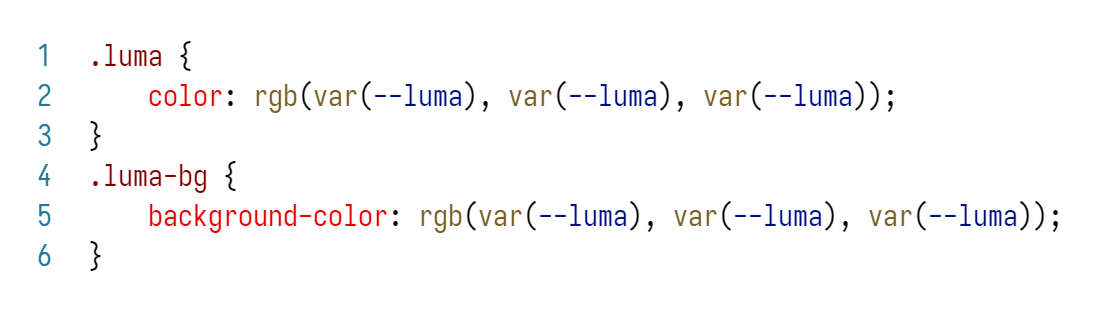
\includegraphics[width=\linewidth]{images/code-css-luma-vars.png}
  \caption{Klasy \texttt{luma} i \texttt{luma-bg}, używające zmiennych \texttt{CSS}}
  \label{fig:css-css-luma-vars}
\end{figure}

Konsekwencją przerzucenia się na taki model jest to, że co wcześniej było ustawieniem jednej klasy, teraz wymaga ustawienia klasy oraz parametru\footnote{Istnieją możliwości pominięcia tworzenia klasy, użwając faktu, że błędne właściwości, np przez korzystanie z niezdefiniownych zmiennych, są ignorowane, lub poprzez przeszukiwanie własności \texttt{style} na elemencie html. Sposoby te mają również swoje wady, więc zdecydowałęm się pozostać przy klasach.}. Tak więc w użyciu, atrybuty na elemencie zmieniają się z \texttt{class="luma-100"} na \texttt{class="luma" style="-\.-luma: 100;"}.

Trzecia z klas w tej samej grupie, \texttt{fix-text}, wymaga nieco większej złożoności w implementacji zamiennika korzystającego ze zmiennych \texttt{CSS}. Ponieważ przetwarzanie zmiennych wewnątrz \texttt{CSS}'u jest bardzo ograniczone, nawet trywialne w innych językach zadania, jak potrzebne tutaj warunkowe wybranie jednej z dwóch wartości, wymaga użycia sztuczek.

Fundamentalnie, do przetwarzania parametrów wewnątrz kodu \texttt{CSS} używa się funkcji \texttt{calc}. Wewnątrz niej, jesteśmy znacznie ograniczeni w tym, jakie operacje możemy przeprowadzić. Najpowszechniej, dostępne jest dodawanie, odejmowanie, mnożenie i dzielenie, oraz funkcje \texttt{min}, \texttt{max} i \texttt{clamp}, łącząca funkcjonalność dwóch poprzednich w jedno. Prócz tego, w nowszych przeglądarkach mamy dostęp do funkcji trygonometrycznych\footnote{\url{https://caniuse.com/mdn-css_types_sin}}, oraz trwają pracę nad ustandaryzowaniem funkcji zaokrąglających\footnote{\url{https://drafts.csswg.org/css-values/\#round-func}}. Dodatkowo, przetwarzanie kolorów jest na moment pisania ograniczone do funkcji mieszającej kolory, \texttt{color-mix}\footnote{\url{https://drafts.csswg.org/css-color-5/\#color-mix}}.

Pomimo tych ograniczeń, jesteśmy w stanie zreplikować wymaganą funkcjonalność. Możemy użyć funkcji generujących kolor, w tym przypadku \texttt{hsl}\footnote{\url{https://drafts.csswg.org/css-color/\#the-hsl-notation}}, aby wygenerować kolory o zdanej światłości. Ponieważ światłość w modelu opisu koloru \texttt{HSL} jest wartością od $0\%$ do $100\%$, wszystkie wartości poniżej $0\%$ będą traktowane jak $0\%$, natomiast wszystko powyżej $100\%$ jako $100\%$. Jeżeli więc stworzymy funkcję, która będzie generowała wartości $\leq 0$ dla wartości parametru \texttt{-\.-luma}, dla której kolorem tekstu ma być czarny, oraz wartości $> 0$ kiedy kolor ten ma być biały, możemy przekazać tą wartość to funkcji koloru \texttt{hsl} po pomnożeniu przez dużą liczbę.

\begin{figure}[H]
  \centering
  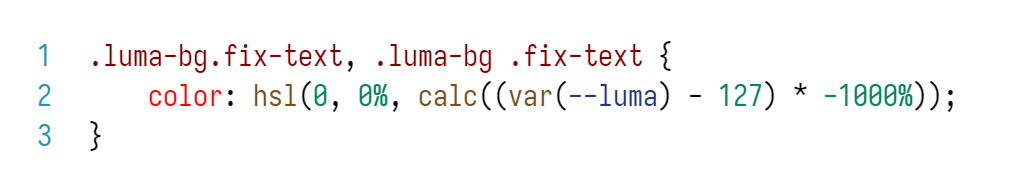
\includegraphics[width=\linewidth]{images/code-css-luma-calc.png}
  \caption{Klasa \texttt{CSS} dokonująca obliczeń, aby wybrać pasujący kolor}
  \label{fig:css-css-luma-calc}
\end{figure}

Patrząc na powyższy kod, możemy przeanalizować, jak on działa, wykonując obliczenia w bloku \texttt{calc}, pamiętając o ograniczeniu zakresu liczbowego funkcji \texttt{hsl}. Gdyby \texttt{var(-\.-luma)} była równa $100$, to otrzymalibyśmy
\[
  \left(100-127\right) \times -1000\% = -27 \times -1000\% = 27000\%
\]
\[
  \min\left(100\%, \max\left(0\%, 27000\%\right)\right) = \min\left(100\%, 27000\%\right) = 100\%
\]
Tak więc dla parametru \texttt{-\.-luma} równemu $100$, otrzymamy kolor \texttt{hsl(0, 0\%, 100\%)}, czyli biały. Wstawiając zamiast $100$ w to samo równanie $128$, czyli wartość, dla której chcemy kolor czarny, otrzymamy

\[
  \left(128-127\right) \times -1000\% = 1 \times -1000\% = -1000\%
\]
\[
  \min\left(100\%, \max\left(0\%, -1000\%\right)\right) = \min\left(100\%, 0\%\right) = 0\%
\]
Można wieć zauważyć, że dla wartości parametru powyżej $127$, wynikiem naszej \texttt{calc}ulacji zawsze będzie $0\%$, natomiast poniżej zawsze $100\%$. Dla niecałkowitych własności parametru \texttt{-\.-luma} ta formuła nie zawsze działa. Np. dla $126.95$ otrzymamy $\left(126.95-127\right)\times-1000\% = -0.05 \times -1000\% = 50\%$, co da nam kolor szary. Można zmniejszyć, jaki duży jest obszar dookoła punktu zmiany między białym a czarny, zwiększająć procentowy mnożnik. Dla $1000\%$, wartości mniejsze od punktu zmiany o mniej niż $0.1$ będą miał to nieporządane zachowanie, gdyż $1000\%\times0.1 = 100\%$. Gdybyśmy chcieli, aby ta akceptowalna różnica od granicy była równa $0.05$, możemy policzyć $\frac{100\%}{0.05} = 2000\%$, co jest naszą wartością dla ujemnego mnożnika w formule.

Mamy już całość funkcjonalności z pliku \texttt{extra.css} zawarte w trzech deklaracjach \texttt{CSS}:

\begin{figure}[H]
  \centering
  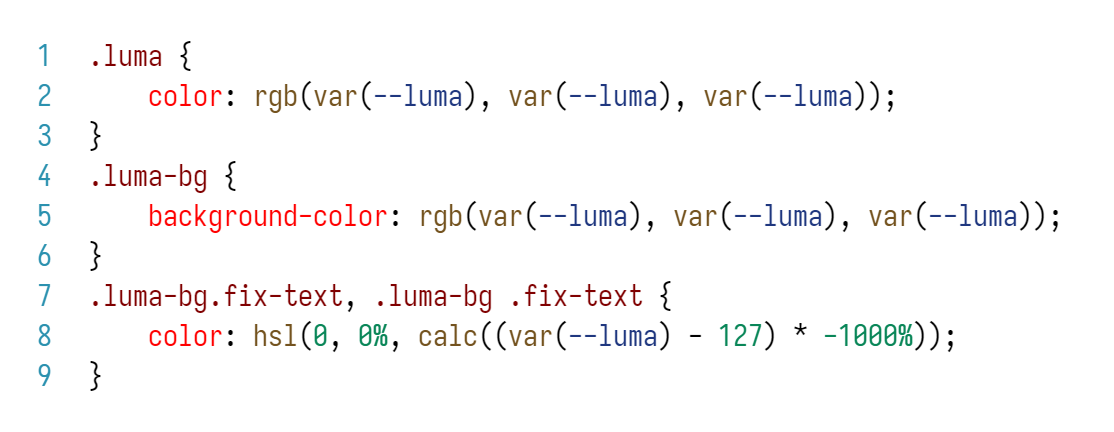
\includegraphics[width=\linewidth]{images/code-css-luma-all.png}
  \caption{Kod \texttt{CSS} zastępujący funkcjonalność klas pomocniczych z pliku \texttt{extra.css}}
  \label{fig:css-css-luma-all}
\end{figure}

Prócz tego musimy dostosować kod generujący elementy do tych zmian. Jeżeli tworzymy nasze elementy za pomocą bezpośrednich API przeglądarki, zmiana ta jest prosta, acz i dla wielu bibliotek ułatwiających tworzenie interfejsów, taka zamiana nie powinna być szczególnie trudna.

\begin{figure}[H]
  \centering
  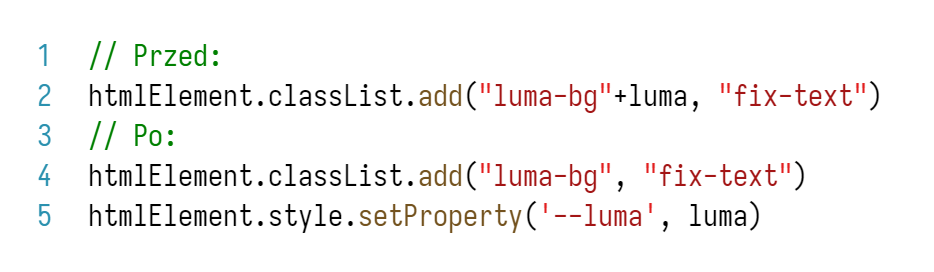
\includegraphics[width=\linewidth]{images/code-js-luma-adjust.png}
  \caption{Zmiana w kodzie \texttt{JavaScript}, który generował elementy korzystające z klas pomocniczych \texttt{luma-\dots}}
  \label{fig:code-js-luma-adjust}
\end{figure}

Kontynuując zamienianie klas pomocniczych na klasy wykorzystujące zmienne \texttt{CSS}, zastąpmy dwie klasy działające wspólnie, \texttt{col-\#} oraz \texttt{row-\#}. Ich działanie polega na stworzeniu siatki w szachownicę, gdzie kolory elementów tej siatki zmieniają się w taki sposób, że elementy po skosie mają ten sam kolor, a elementy ortagonalnie przykległe zmieniają go.

\begin{figure}[H]
  \centering
  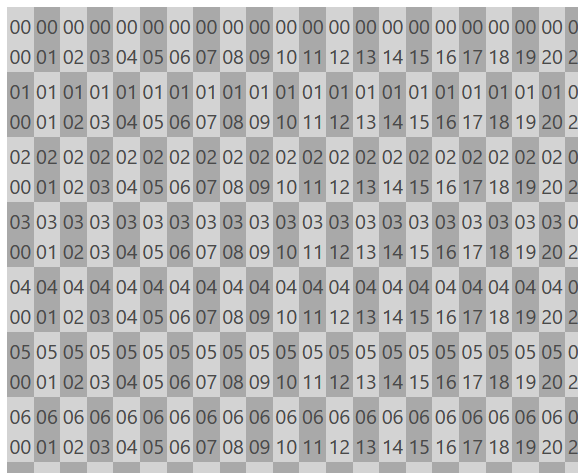
\includegraphics[width=\linewidth/\real{1.2}]{images/ui-grid-darken.png}
  \caption{Efekt, który chcemy uzyskać}
  \label{fig:ui-grid-darken}
\end{figure}

Morzemy skorzystać z \texttt{CSS}'owej pseudoklasy \texttt{:nth-child()}. Jest ona uniwersalnie wspierana\footnote{\url{https://caniuse.com/mdn-css_selectors_nth-child}}, i pozwala na wybieranie elementów po ich kolejności na bazie formuły matematycznej. Ponieważ siatka na stronie składa się z elementu zawierającego wiersze, które to zawierają komórki, możemy prosto naprzemiennie pokolorować parzyste i nieparzyste wiersze.

\begin{figure}[H]
  \centering
  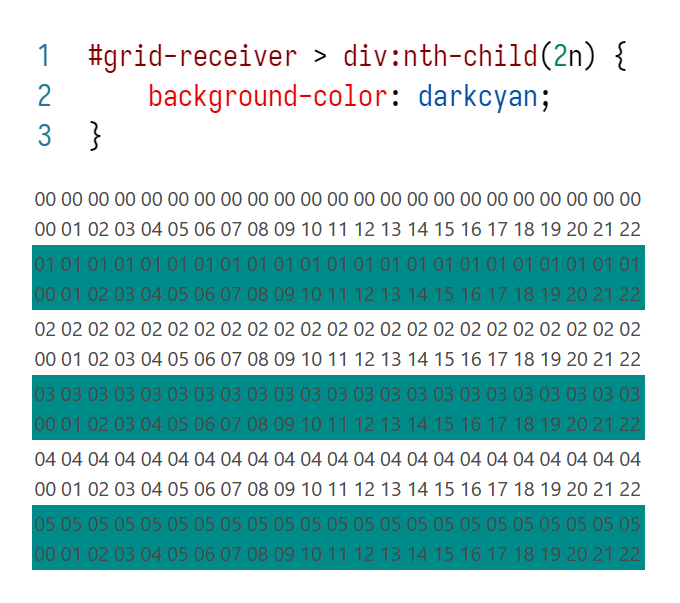
\includegraphics[width=\linewidth/\real{1.6}]{images/codeui-row-coloring.png}
  \caption{Fragment kodu oraz efekt, jaki ma on na siatkę. Warto zwrócić uwagę, że liczenie kolejności elementu zaczyna się od $1$, nie od $0$, więc wiersze pod nieparzystymi indeksami według kodu JavaScript są parzyste według \texttt{CSS}}
  \label{fig:codeui-row-coloring}
\end{figure}

Możemy więc wybrać dla tych wierszy tylko ich parzyste komórki, oraz dodać kod wybierające nieparrzyste komórki nieparzystych wierszy.

\begin{figure}[H]
  \centering
  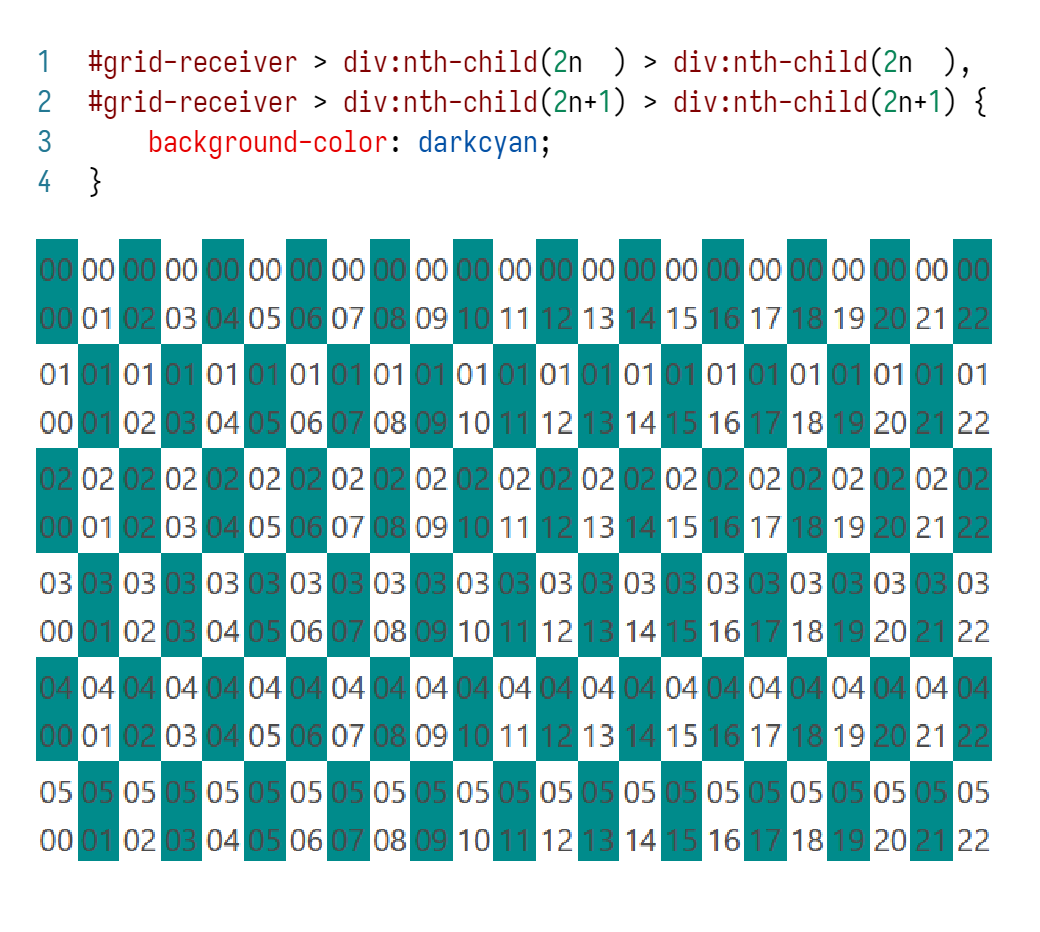
\includegraphics[width=\linewidth/\real{1.6}]{images/codeui-checkerboard-half-coloring.png}
  \caption{Stylowanie połowy szachownicy w siatce}
  \label{fig:codeui-checkerboard-half-coloring}
\end{figure}

Następnie, możemy dodać kod do przeciwnych wypadków, czyli parzystych komórek nieparzystych wierszy oraz nieparzystych komórek parzystych wierszy.

\begin{figure}[H]
  \centering
  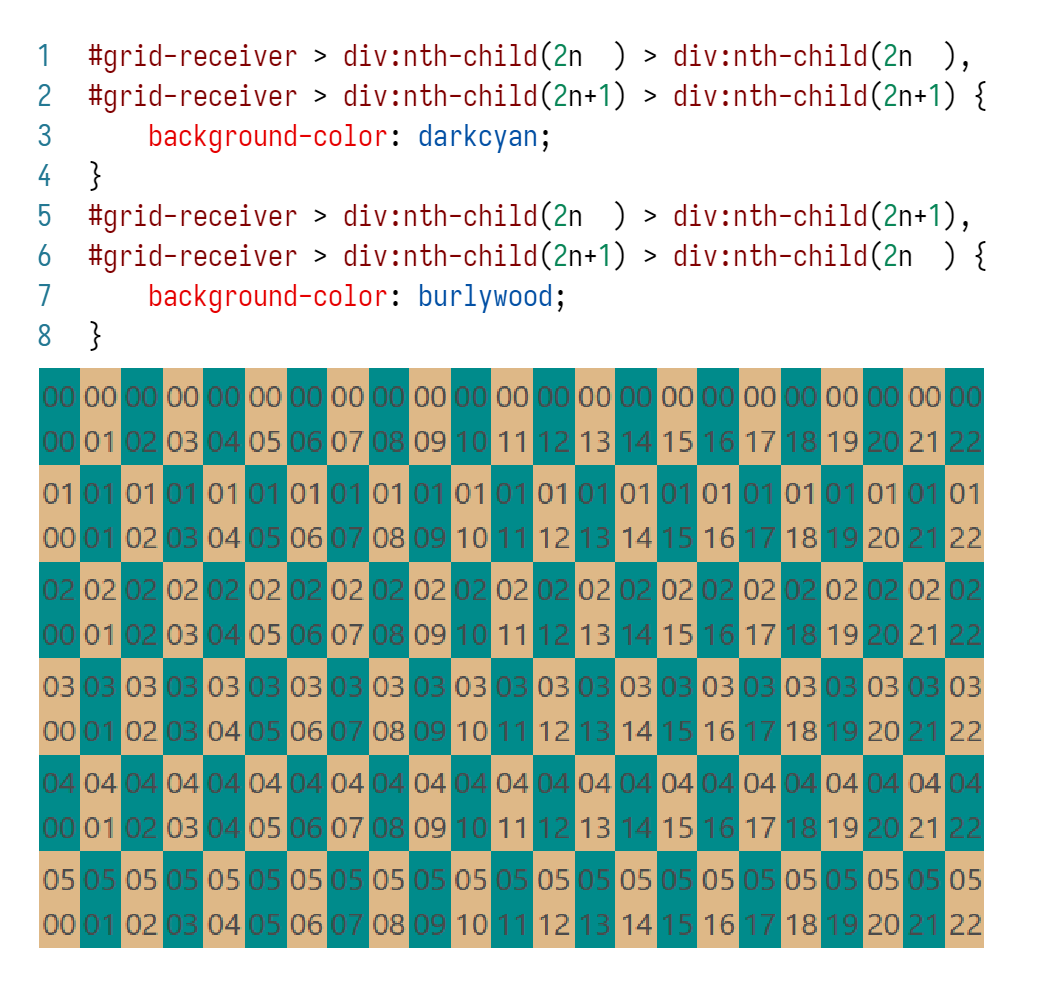
\includegraphics[width=\linewidth/\real{1.6}]{images/codeui-checkerboard-coloring.png}
  \caption{Stylizowanie całości szachownicy}
  \label{fig:codeui-checkerboard-coloring}
\end{figure}

Mając ten kod, wystarczy wybrać kolory chcemy, i działanie skończone. Niestety, takie rozwiązanie ma problem, nad rozwiązaniem którego są aktywnie prowadzone prace\footnote{\url{https://drafts.csswg.org/selectors/\#example-3c07f717}}, a jest nim to, że nie możemy wykluczyć elementów z bycia uwzględnianymi w liczeniu parzystości. Gdyby więc mieć w takiej siatce wiersze niebędące częścią szachownicy, np. separatory między różnymi przedstawianymi zbiorami, zaburzałyby one dopasowania do naszej formuły parzystości. Od niedawna dostępna jest opcja dodania selektora \texttt{CSS}, który określa, które z elementów mają być uzwględniane do liczenia tej formuły, i choć funkcja ta jest szeroko wspierana\footnote{\url{https://caniuse.com/css-nth-child-of}}, jest dalej nowa, a jej standaryzacja niezakończona.

Kolejnym elementem optymalizacji \texttt{CSS} który możemy zrobić, to wycięcie z biblioteki Bulma tylko tych części, które potrzebujemy. Na szczęście dla nas, Bulma wspiera proste tworzenie własnych jej wersji poprzez skorzystanie języka \texttt{Scss}, który jest rozszerzeniem \texttt{CSS}. Możemy więc zaimportować tylko części biblioteki, z których chcemy korzystać, i skompilować je do pliku \texttt{CSS}.

\begin{figure}[H]
  \centering
  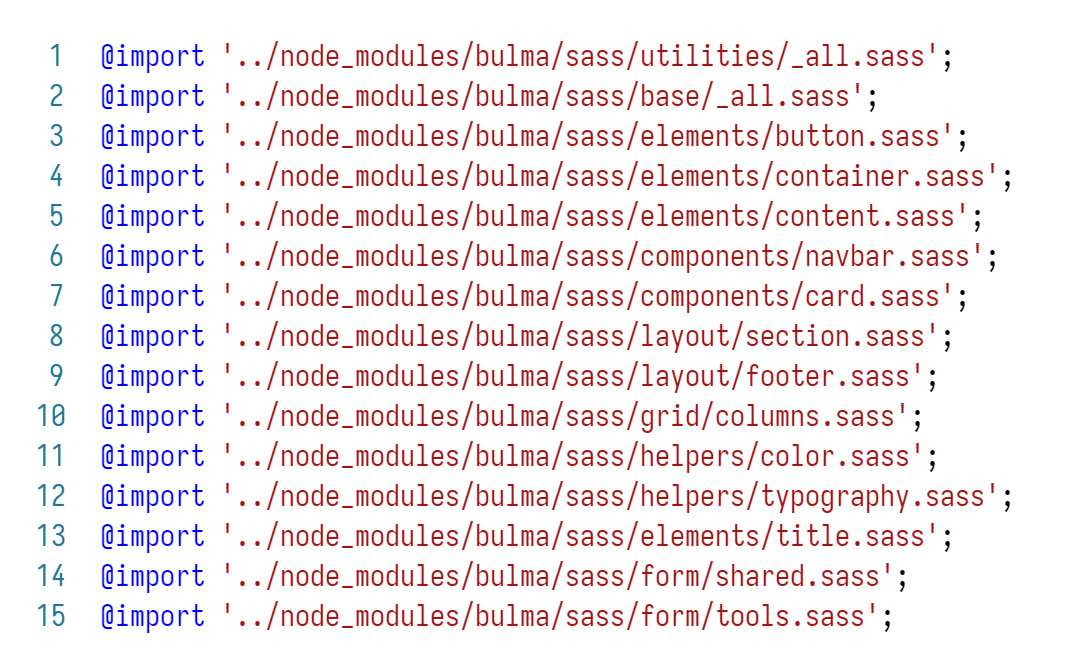
\includegraphics[width=\linewidth]{images/code-scss-import-bulma.png}
  \caption{Plik \texttt{Scss} importujący fragmenty biblioteki Bulma, wybierając tylko używane na stronie jej elementy}
  \label{fig:code-scss-import-bulma}
\end{figure}

Ponieważ sami budujemy pliki biblioteki, oraz ponieważ plik \texttt{extra.css} stał się teraz bardzo mały, możemy połączyć je w jeden plik, który będzie spełniał funkcję ich obu. Pomoże to ze stałym kosztem przesyłania danych drzewa Huffmana na początku skompresowanych \texttt{gzip}'em plików, oraz zredukuje ilość równoległych połączeń.

Na końcu możemy dokonać minifikacji generowanych plików \texttt{CSS}. Minifikacja polega na usunięciu pomocnych dla czytelności białych znaków z miejsc, gdzie nie mają one znaczenia dla treści \texttt{CSS}'owych definicji. Możemy do tego użyć narzędzi jak \href{https://www.npmjs.com/package/uglifycss}{uglifycss}, które można użyć z wiersza polecenia lub skryptu \texttt{JavaScript}.

Uruchamiając test WebPageTest'u, otrzymujemy następujące wyniki:

\begin{figure}[H]
  \centering
  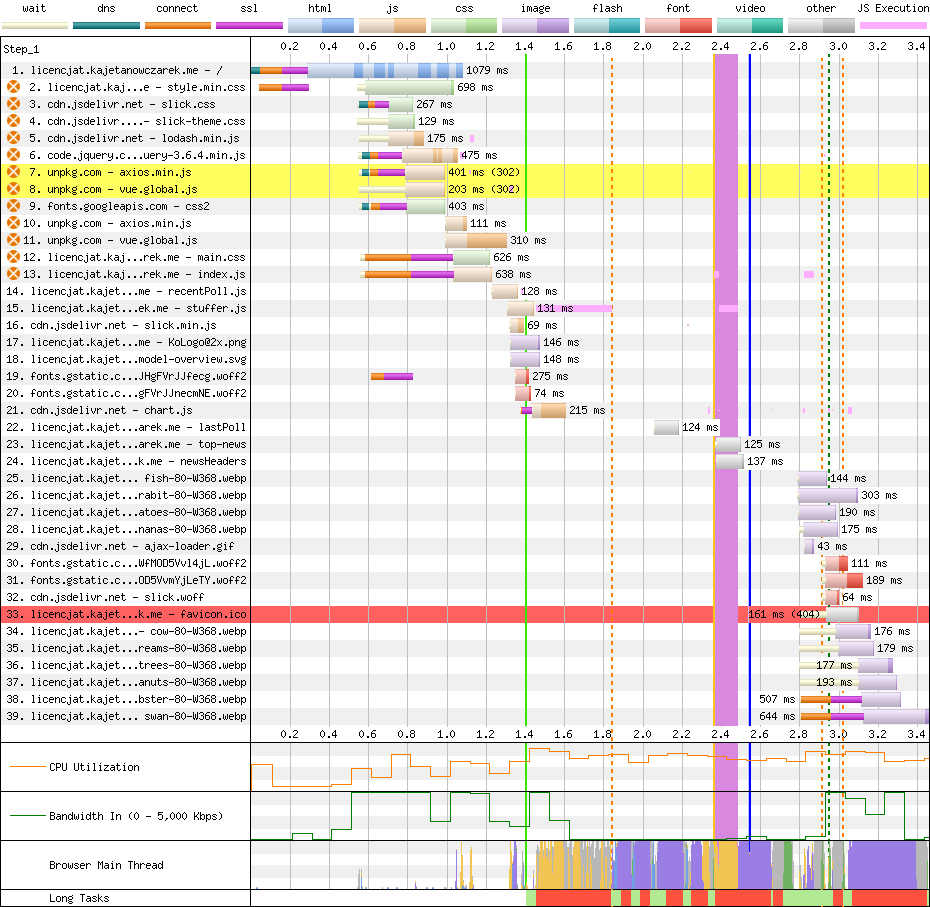
\includegraphics[width=\linewidth]{images/waterfall-after-css.png}
  \caption{Wyniki po poprawieniu plików \texttt{CSS}}
  \label{fig:waterfall-after-css}
\end{figure}

Porównując z poprzednimi wynikami, to choć witryna wczytuje się łącznie wręcz nieco dłużej, o około $0.11$ sekundy, tak rozpoczęcie renderowania ma miejsce około $0.2$ sekundy wcześniej. Oznacza to, że użytkownicy wcześniej dostają jakąś treść na ekranie, ale po tych specyficznych zmianach musimy poczekać nieco dłużej na pełne wczytanie się zdjęć. Mimo to, szybsze wyświetlenie zawartości strony jest warte dla nas więcej, niż przyśpieszenie momentu jej pełnej gotowości.

\section{Wczytywanie treści HTML asynchronicznie}

Następnym elementem powstrzymującym naszą witrynę przed byciem widoczną i używalną jest duży i wolno wczytujący się główny plik \texttt{html}. Jego rozmiar wynika z tego, że zawiera on bardzo dużą ilość treści, przez co strona jest bardzo długa, i znaczna część jej prezentowalnej zawartości jest daleko poza wstępnym widokiem. Możemy więc opóźnić wczytywanie tej treści do momenty po tym, jak wczyta się pierwszy widok na stronie.

Metodą, którą możemy użyć do wczytywania treści \texttt{html} w sposób szybki i wydajny, to używając możliwości strumieniowania połączeń tworzonych przez funkcję \texttt{fetch} oraz tworząc dodatkowe instancje dokumentów html.

Podstawowym konceptem, który wykorzystamy, to tworzenie nowych, częściowych dokumentów przy użyciu funkcji \texttt{document.implementation.createHTMLDocument}. Pozwala nam ona stworzyć dokument przeglądarki, który nie jest powiązany z żadnym oknem lub kontekstem renderowania, więc podczas dodawania do niego treści nie będą dokonywane obliczenia układu strony lub wczytywanie treści wizualnych. Możemy więc, używając \texttt{document.write} na stworzonym przez nas dokumencie wstawiać w niego nowy kod \texttt{html} w trakcie, gdy jest on pobierany.

Aby nałożyć na siebie pobieranie, dekodowanie i interpretowanie danych, możemy użyć systemu strumieni. Używając funkcji \texttt{fetch}, aby pobrać dane z serwera, możemy po nawiązaniu połączenia użyć właściwości \texttt{body} na obiekcie odpowiedzi, aby uzyskać dostęp do strumienia przychodzących danych. Strumień ten składa się z niezinterpretowanych bajtów, które musimy przekonwertować na tekst przy użyciu danego kodowania. Możemy to osiągnąć za pomocą obiektu klasy \texttt{TextDecoderStream}, na którego strumień wejścia można wysyłać sekwencje bajtów, a on na swoim stumieniu wyjścia będzie emitował kolejne \texttt{string}'i. 

Łącząc te koncepty w całość, otrzymujemy następujący kod:

\begin{figure}[H]
  \centering
  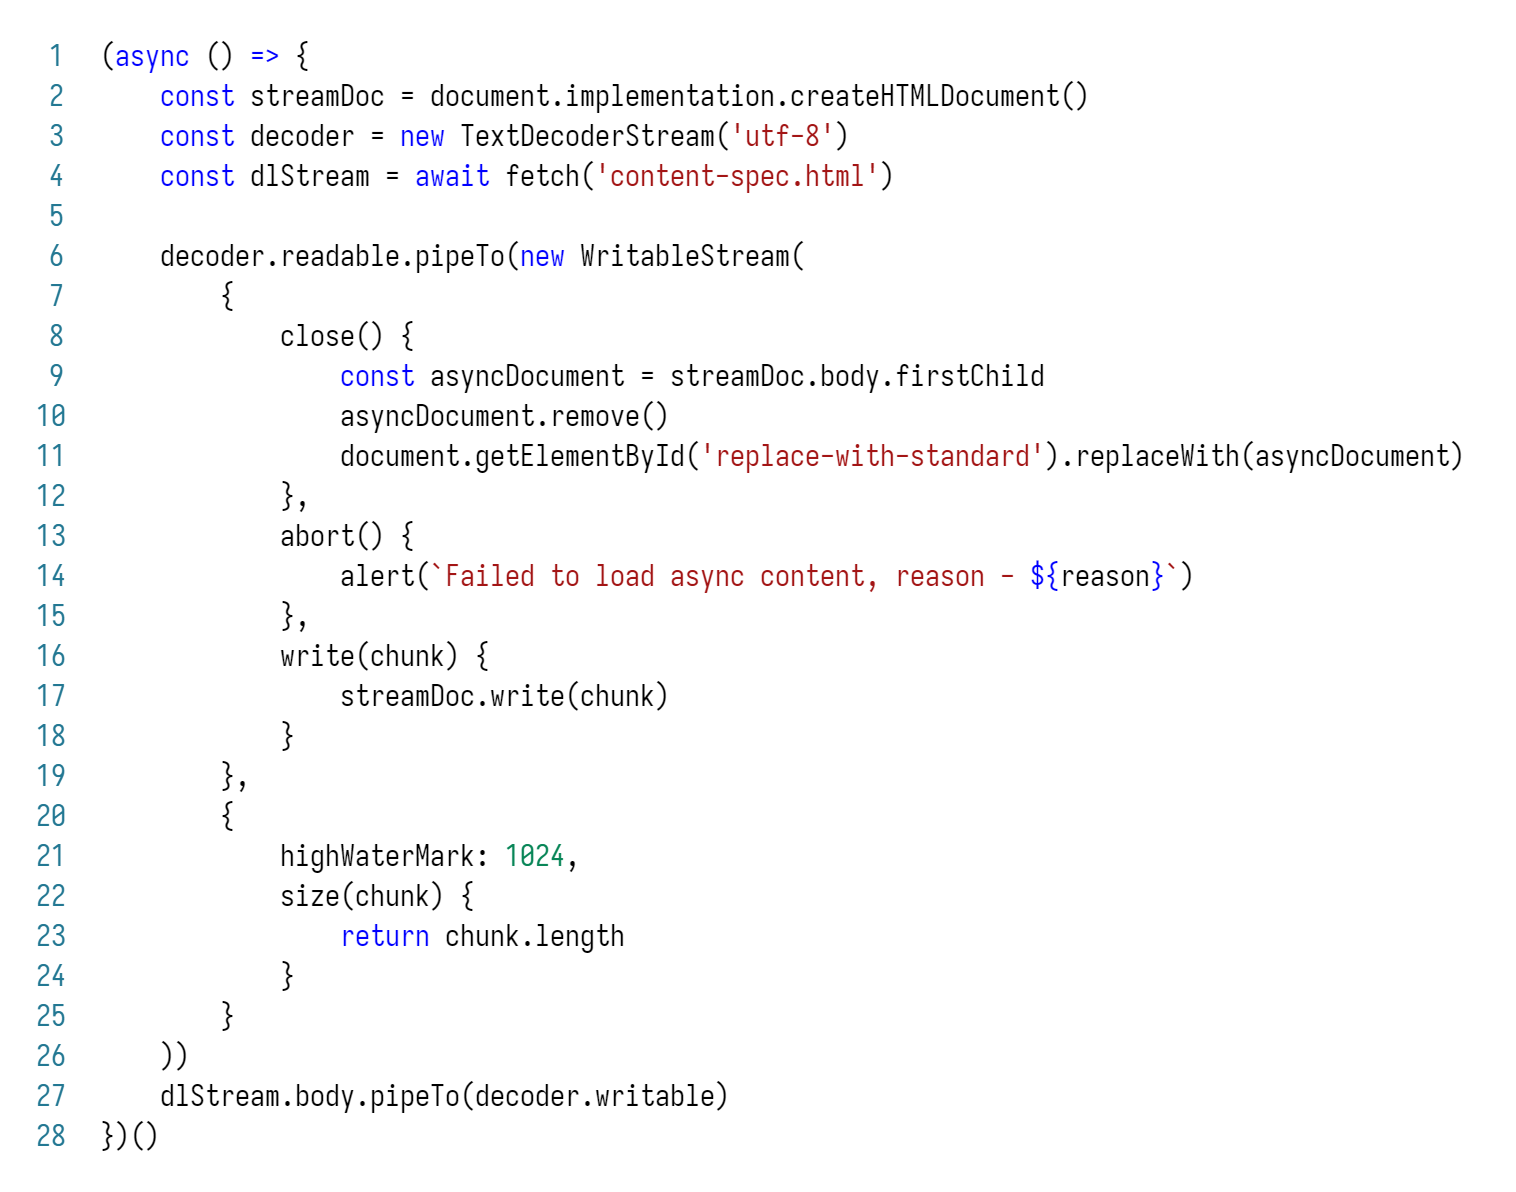
\includegraphics[width=\linewidth]{images/code-js-async-streaming.png}
  \caption{Kod wczytujący zasób \texttt{content-spec.html} w sposób asynchroniczny, a następnie wstawiający wczytaną zawartość do treści witryny}
  \label{fig:code-js-async-streaming}
\end{figure}

Dodjąc ten kod do strony, i zastępując treści z pliku \texttt{index.html}, która teraz będzie wczytywana, elementem o \texttt{id} \texttt{replace-with-standard}, a następnie testując wydajność witryny po zmianach, otrzymujemy następujące wyniki:

\begin{figure}[H]
  \centering
  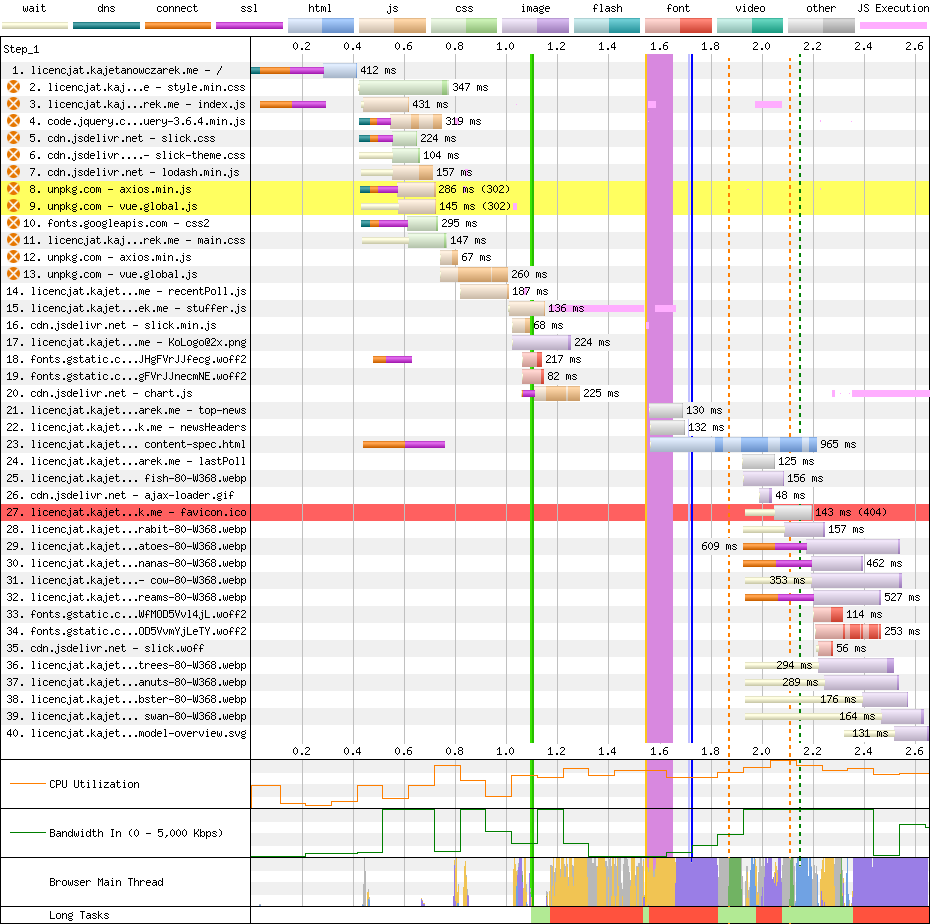
\includegraphics[width=\linewidth]{images/waterfall-after-async-html.png}
  \caption{Wyniki pomiarów po wdrożeniu asynchronicznego wczytywanie dużych treści \texttt{html}}
  \label{fig:waterfall-after-async-html}
\end{figure}

Porównując te wyniki, otrzymaliśmy wielką poprawę dla łącznego czasu wczytywania oraz rozpoczęcia renderowania. Czas do pierwszej treści na ekranie spadł z $1.4$ sekundy na $1.05$ sekund, co jest poprawą o $25\%$, a łączny czas wczytywania witryny - z $3.4$ do $2.6$ sekund. Zyskaliśmy więc znacznie na obu rodzajach szybkości wczytywania, i zbliżamy się do przełamania $1$ sekundy do pierwszego obrazu.

\section{Redukcja kodu JavaScript}



\chapter{Zakończenie}

\begin{thebibliography}{7}
\addcontentsline{toc}{chapter}{Bibliografia}
%
\bibitem{Lang}
Serge Lang, 
\textit{Algebra. Revised third edition}, 
New York, Springer-Verlag, 2002.
%
\bibitem{Kostrykin} 
Aleksiej Kostrykin, 
\textit{Wstęp do algebry. Podstawy algebry},
Warszawa, Wydawnictwo Naukowe PWN, 2022.
\end{thebibliography}
\end{document}